\chapter{基于局部加权矩阵分解的商品推荐}
\label{chapter-lwmf}
本章主要介绍针对隐式反馈数据上进行商品推荐的研究工作。首先,章节~\ref{sect-lwmf-intro}阐述本章的研究背景、研究问题、研究主要贡献等。其次,章节~\ref{sec-lwmf-lwmf}重点介绍本章提出的模型,包括模型框架、优化算法等。随后,章节~\ref{sec-lwmf-exp}分析基于公开真实世界数据集上的实验结果。最后小结本章商品推荐的研究内容。

\section{引言}
\label{sect-lwmf-intro}


\textit{商品推荐}是推荐系统中的主要任务,是根据用户的历史行为数据,刻画用户画像,帮助人们在海量商品中发现他们感兴趣的商品。而用户的历史数据中按照用户的行为分为显式反馈数据和隐式反馈数据。其中显式反馈数据指的是用户在访问商品(例如购买商品,观看电影,餐馆用餐等行为)之后对商品进行评分表达自己的满意程度,标注标签表达商品的特性以及进行文本评价表明自己的体验感受。而隐式反馈数据指的是用户访问商品之后行为产生的非显式反馈的数据。因为显式反馈数据需要用户额外花一些时间进行评价,所以用户产生的大部分数据都属于隐式反馈。本章主要研究在隐式反馈数据集上的\textit{商品推荐}。

隐式反馈数据中,对于用户访问过的商品,次数代表了用户对商品的感兴趣程度,可以作为正反馈样例。大多数用户未访问过商品的数据对学习用户特征也是有帮助的,一般可以作为负反馈样例,但是次数为0代表了两种情况:(1)用户对这类商品不感兴趣;(2)用户对这类商品感兴趣,但还未发现此类商品。因此Hu等人~\cite{hu2008collaborative}提出了加权矩阵分解(Weighted Matrix Fatorization,简称WMF),访问次数大于0的数据为正反馈样本,次数等于0的样本为负样本,而次数则以权重的形式加入矩阵分解中(访问次数越多,权重越大,说明访问次数大于0的数据为正反馈样本的概率越大)。具体地,WMF已经在章节~\ref{sec-related-wmf}详细阐述。因为WMF模型是将用户和商品投射到潜在的低维空间,所以它的一个前提假设是隐式反馈数据中次数数据矩阵是全局低秩的。最近,Lee等人\cite{lee2013local,lee2014local}认为显式评分数据不是全局低秩的,而局部评分矩阵是低秩,拥有局部信息,通过对评分矩阵中的局部子矩阵进行建模能够得到更好的评分预测效果。类似的工作还有WEMAREC~\cite{chen2015wemarec}。本文统称这类工作为局部矩阵分解。如图~\ref{fig-lwmf-lmf}所示,局部矩阵分解模型首先将原始矩阵划分为若干更小的子矩阵,每个子矩阵内的用户(商品)之间是相互关联的,用来表示矩阵内的局部结构,然后利用标准的矩阵分解模型将每个子矩阵的用户和商品投射到隐藏空间,最后利用加权平均求和来预测最终的评分值。因此局部矩阵分解模型就可以利用局部结构特征来获得比原始矩阵分解更好的低秩近似。

\begin{figure}
	\centering
	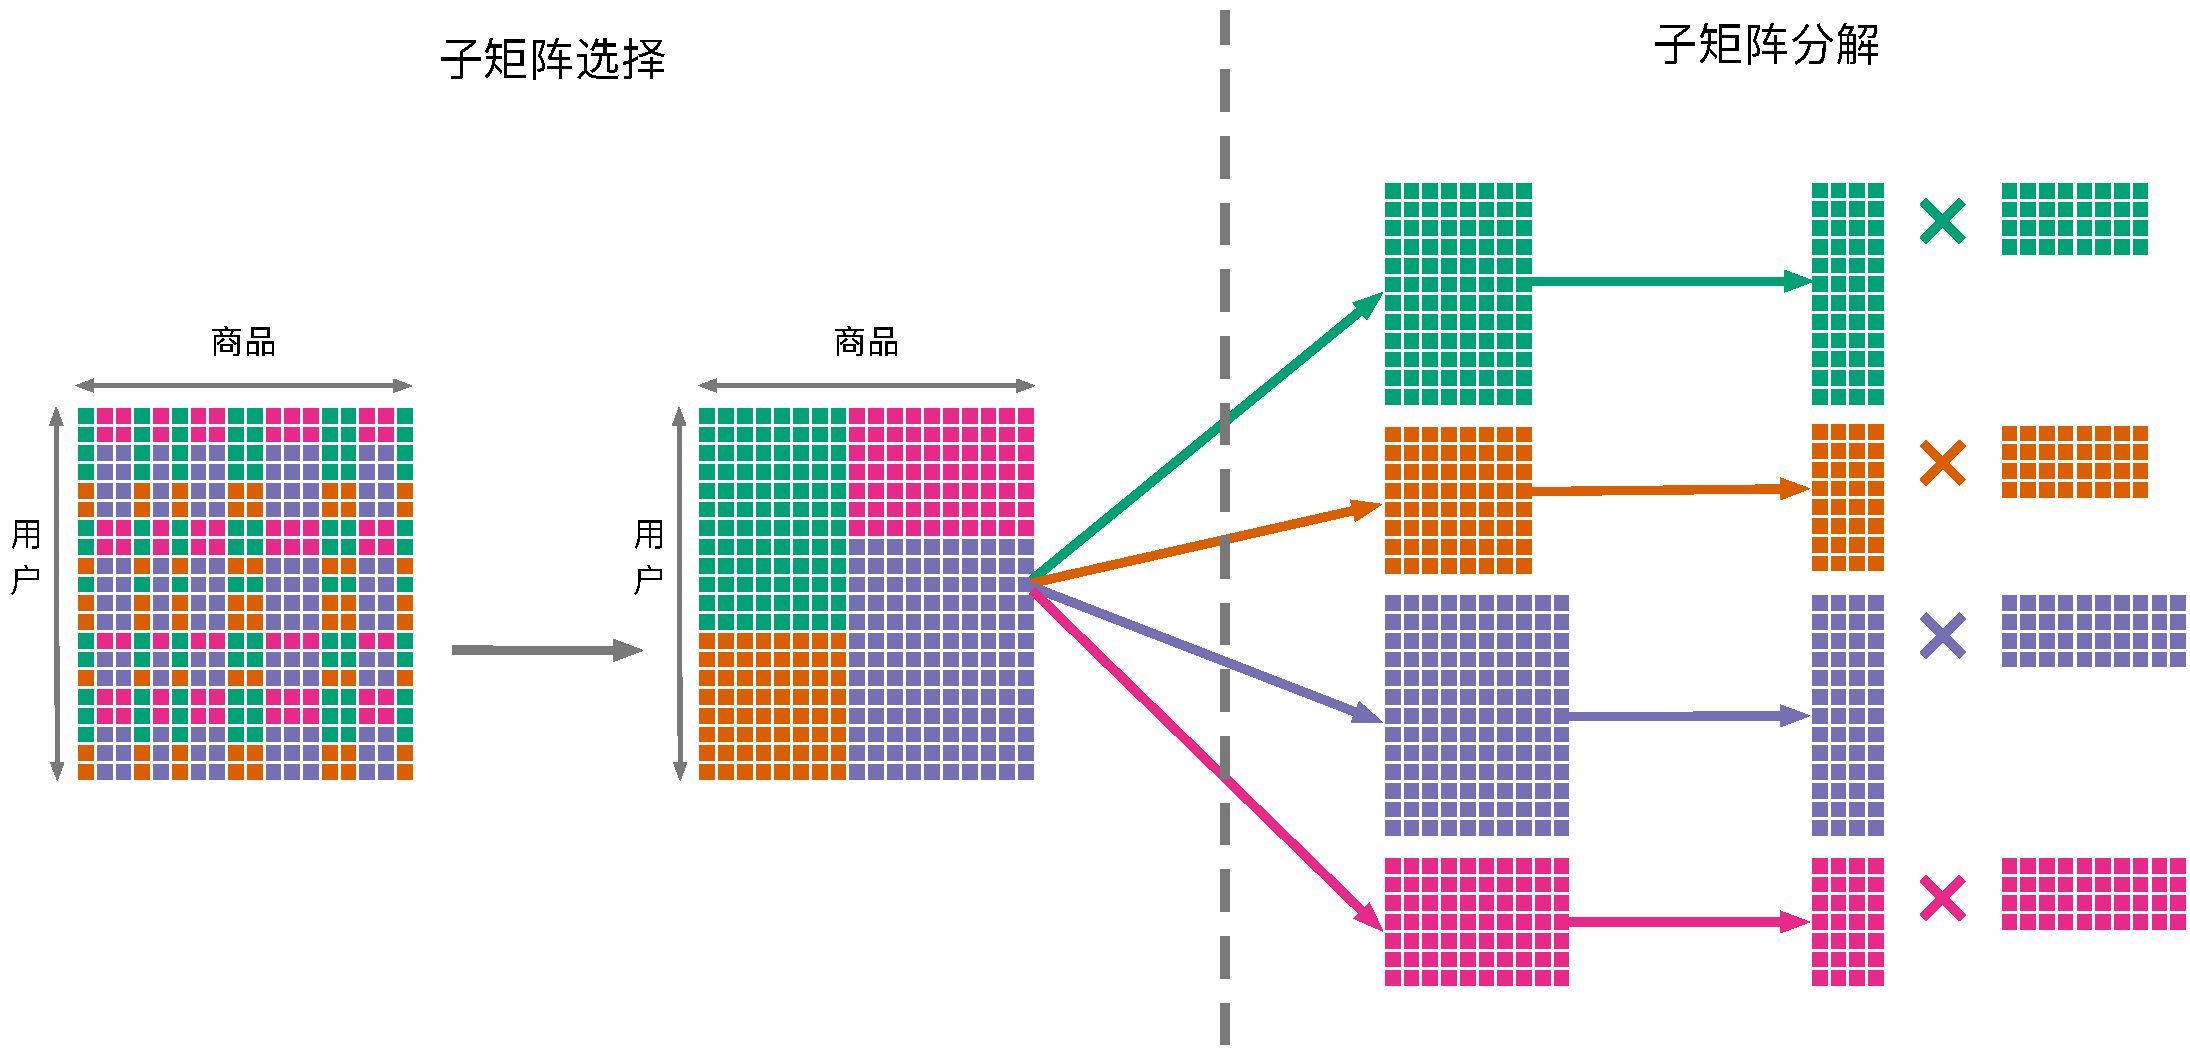
\includegraphics[width=1.0\textwidth]{Fig/lwmf/lmf}	
	\caption{局部矩阵分解模型}
	\label{fig-lwmf-lmf}
\end{figure}

考虑到隐式反馈数据和显式反馈数据的相似性,本章节也认为隐式反馈数据不是全局低秩的,而是局部低秩的,考虑在隐式反馈数据集上对数据的局部性质建模,进行个性化\textit{商品推荐}。例如,根据用户的签到数据集进行兴趣点(Point Of Interests,简称POI)推荐,因为兴趣点天然地具有地理信息这一特征,用户更倾向于访问与自身相近的地点,所以在同一个区域的用户访问的兴趣点比不在同一个区域的用户所访问的兴趣点更加类似。

因此,本章节设计了加权局部矩阵分解(Local Weighted Matrix Factorization,简称LWMF), 将LLORMA~\cite{lee2013local,lee2014local}和WMF~\cite{hu2008collaborative}相结合,使用核函数来寻找子矩阵和建立权重函数来建模用户局部偏好和商品的局部特性,提高商品推荐的准确率。这种方法也带来两个好处,(1)因为子矩阵的密度比原始矩阵要高很多,隐式数据中正反馈数据的稀疏性问题得到了一定程度的缓解;(2)子矩阵之间的分解可以并行进行,使得模型更加容易并行化。


具体地,本章主要贡献总结如下:
\begin{itemize}
	\item 本章节工作结合了LLORMA和WMF,提出了加权局部矩阵分解模型(LWMF),在隐式反馈数据上进行商品推荐。 LWMF通过将原始矩阵划分为子矩阵来对矩阵进行局部建模,并且缓解了访问次数数据的稀疏性问题以及使得矩阵分解模型更加容易并行化、分布式地进行模型训练。
	\item 为了更好地近似原始矩阵,本章节工作在基于核函数的方法上,提出DCGASC(折扣累积增益锚点集合覆盖)来选择子矩阵。同时,本章节工作还从理论上对DCGASC目标函数的次模性质和单调性进行分析,证明利用贪心算法能够以$1-\frac{1}{e}$得到近似最优解。
	\item 基于商品推荐问题,本章节⼯作进⼀步提出了两种变体方法:基于⽤户的 LWMF和基于商品的 LWMF,其中基于用户的LWMF对商品推荐更为合理,能够获得更好的性能。
	\item 本章节工作在真实数据集上进行充分的实验,在各个维度上比较了LWMF与WMF算法,实验结果表明了本章节模型的有效性。
\end{itemize}





\begin{table}
	\centering
	\caption{本章主要符号说明}
	\label{tab-lwmf-notation}%
	
	\begin{tabular}{cp{0.68\columnwidth}}
		\hline
		符号 & 符号描述 \bigstrut \\
		\hline\hline
		$\mathbf{R}^h$ & 第$h$个子数据矩阵 \bigstrut\\
		$\mathbf{C}^h$ &第$h$个01(二值化)化子数据矩阵  \bigstrut\\
		$ \mathbf{W}^h$ &01(二值化)化子数据矩阵$\mathbf{C}^h$的置信权重矩阵\bigstrut\\
		$ \mathbf{V}^h$ & 01(二值化)化子数据矩阵$\mathbf{C}^h$的子矩阵权重矩阵 \bigstrut\\
		$ \mathcal{P}^h$ &第$h$个数据子矩阵中的用户索引集合  \bigstrut\\
		$ \mathcal{Q}^h$ &第$h$个数据子矩阵中的商品索引集合  \bigstrut\\
		$ \mathbf{P}^h$  & 子数据矩阵$\mathbf{R}^h$中用户局部隐藏特征矩阵 \bigstrut\\
		$\mathbf{Q}^h$  & 子数据矩阵$\mathbf{R}^h$中商品局部隐藏特征矩阵 \bigstrut\\
		\hline
		$ \mathcal{\hat{A}}$ & 锚点集合($\subset \mathcal{A}$) \bigstrut\\
		$\hat{a}_h=\langle\hat{u}_h, \hat{m}_h\rangle$ & 锚点  ($\in \mathcal{\hat{A}}$)   \bigstrut\\
		$E(a_i, a_j)$ & 两个数据点之间的核函数值 \bigstrut\\
		$b$ & 核函数宽度参数 \bigstrut\\
		\hline
	\end{tabular}
\end{table}


\section{模型描述与优化}
\label{sec-lwmf-lwmf}
本章节首先介绍本章提出的针对隐式反馈数据的\textit{商品推荐}模型,称为局部加权矩阵分解(Local Weighted Matrix Factorization ,简称LWMF)。随后,本章设计了一个启发式的算法去选择子矩阵,提取数据矩阵的局部信息。最后,为了学习局部隐藏特征矩阵$\mathbf{P}^h$和$\mathbf{Q}^h$,本章还改进了交替最小二乘优化算法以适用于LWMF参数的快速学习。表\ref{tab-lwmf-notation}中列出了本章节中使用的符号表。基础的符号描述见表\ref{tab-basic-notation}中所示。矩阵和集合的字符的小写上标,例如$\mathbf{R}^h$和$\mathcal{P}^h$,表示不同的子矩阵以及相应用户索引集合。

\subsection{模型概览}
类似于LLORMA~\cite{lee2013local,lee2014local},LWMF模型首先从原始数据矩阵选择子矩阵,然后利用WMF对子矩阵进行矩阵分解。具体的WMF模型见章节\ref{sec-related-wmf}。本章结合了LLORMA和WMF在隐式反馈数据集上进行\textit{商品推荐},提出了局部加权矩阵分解,利用WMF对第$h$个二值化数据子矩阵$\mathbf{C}^h$进行如下分解:

\begin{equation}
\min_{\mathbf{P}_h,\mathbf{Q}_h}\sum_{u=1}^{N}\sum_{m=1}^{M}\mathbf{V}_{um}^h\mathbf{W}_{um}^h(\mathbf{C}_{um}^h-{\mathbf{P}_{u}^h}^\top \mathbf{Q}_{m}^h)^2+\lambda_\mathbf{P}^h\|\mathbf{P}^h\|_F^2+\lambda_\mathbf{Q}^h\|\mathbf{Q}^h\|_F^2
\end{equation}
其中$\lambda_\mathbf{P}^h$和$\lambda_\mathbf{Q}^h$ 是子矩阵用户和商品的正则化因子。原始二值化数据矩阵$\mathbf{C}$可以被一系列子矩阵集合$\mathcal{C}= \{\mathbf{C}^1,\mathbf{C}^2,...,\mathbf{C}^H\}$所组成:

\begin{equation}
\mathbf{C}_{um} \approx \frac{1}{\mathbf{Z}_{um}}\sum_{h=1}^H \mathbf{V}_{um}^h{\mathbf{P}^h_u}^\top \mathbf{Q}^h_m
\end{equation}
其中$\mathbf{Z}_{um} = \sum_{h=1}^H \mathbf{V}_{um}^{h}$是归一化因子,$\mathbf{V}^{h}_{um}$ 代表在子矩阵$\mathbf{C}^{h}$中项$\mathbf{C}^{h}_{um}$的权重。从上述公式可以看出,此类子矩阵集成分解的两个关键问题是(1) 如何选择和生成子矩阵?(2) 如何设置子矩阵的权重和根据子矩阵近似原始矩阵?

类似于LLORMA的子矩阵选择方法,本章节工作首先在数据集合$\mathcal{A}=\{a_1, a_2, ..., a_{|\mathbf{R}|}\}$ 中找一个数据点$a_i=\langle u_i, m_i \rangle$作为锚点$\hat{a}_h=\langle\hat{u}_h, \hat{m}_h\rangle$。然后利用相似度计算方法或者核函数计算锚点和其他数据点之间的相关程度。最后,选择那些相关程度大于一定常数的数据点组成子矩阵。可以看出,子矩阵中的数据点之间是相似的。另外,只要使用上述方法选择更多的锚点,从而得到更多的子矩阵。

实际上,本章工作使用Epanechnikov核函数去计算两个数据点$a_i=(u_i,m_i)$和$a_j = (u_j,m_j)$之间的相关程度。具体地,本章利用Epanechnikov核函数计算用户之间的相关程度和商品之间的相关程度,然后将它们的乘积作为数据点$a_i=(u_i,m_i)$和$a_j = (u_j,m_j)$之间的相关程度,具体如下表示:

\begin{eqnarray}
\mathit{E}(a_i, a_j)=\mathit{E_{b}}(u_i, u_j)\times\mathit{E_{b}}(m_i, m_j)
\end{eqnarray}
其中$\mathit{E_{b}}(u_i, u_j)$和$\mathit{E_{b}}(m_i, m_j)$是Epanechnikov核函数,

\begin{eqnarray}
	\mathit{E_{b}}(u_i, u_j)&\varpropto&(1-d(u_i,u_j)^2) \,\mathbf{1}_{\{d(u_i,u_j)\leq {b}\}}\nonumber\\
	\mathit{E_{b}}(m_i, m_j)&\varpropto&(1-d(m_i,m_j)^2) \,\mathbf{1}_{\{d(m_i,m_j)\leq {b}\}}\nonumber
\end{eqnarray}
其中$b$是核函数的宽度参数。两个用户(或者商品)的距离利用两个用户(或者商品)的隐藏特征向量计算。初始的用户隐藏特征向量和商品隐藏特征向量从数据矩阵$\mathbf{R}$中利用WMF中学习得到。对应地,本章工作利用$d(u_i, u_j)=arccos(\frac{\mathbf{P}_{u_i}\cdot \mathbf{P}_{u_j}}{\|\mathbf{P}_{u_i}\|\cdot\|\mathbf{P}_{u_j}\|})$ 计算用户$u_i$和$u_j$之间的距离,其中$\mathbf{P}_{u_i}$, $\mathbf{P}_{u_j}$就是第$u_i$个用户和第$u_j$个用户的全局隐藏特征向量。同理,使用同样的方法计算商品之间的距离。因此在选定锚点$\hat{a}_h=\langle\hat{u}_h, \hat{m}_h\rangle$ 的前提下,本章工作在子矩阵$\mathbf{R}^h$中设置用户商品对$\langle u_j,m_j \rangle$的权重为$\mathbf{V}^h_{u_jm_j} = \mathit{E}(\hat{a}_h, a_j)$ ,同时子矩阵的正则化参数变为$\lambda_\mathbf{P}^h = \lambda_\mathbf{P} \mathit{E_{b}}(\hat{u}_h, u_j)$和 $\lambda_\mathbf{Q}^h=\lambda_\mathbf{Q} \mathit{E_{b}}(\hat{m}_h, m_j)$。

从上述选择子矩阵的方法可以看出,每选出一个锚点就代表一个子矩阵。选择子矩阵集合$\mathcal{C}$实际上就是选择一个锚点集合$\hat{\mathcal{A}}=\{\hat{a}_1, \hat{a}_2, ..., \hat{a}_H\}$。 具体地,将在下一小节讨论选择锚点集合的算法。

\subsection{锚点集合选择}
\label{sec-lwmf-asc}
直观地,子矩阵集合$\mathcal{C}= \{\mathbf{C}^1,\mathbf{C}^2,...,\mathbf{C}^H\}$ 应该需要覆盖整个原始二值化矩阵$\mathbf{C}$,也就是说$\mathbf{C} = \cup_{\mathbf{C}^h\in \mathcal{C}}\mathbf{C}^h $。因此那些能够覆盖原始矩阵的子矩阵集合$\mathcal{C}$ 一般能够比不能覆盖原始矩阵的子矩阵集合更好地近似原始矩阵$\mathbf{C}$ 。因此,锚点集合选择问题就变成锚点集合覆盖问题。

\subsubsection{简单锚点集合覆盖}
\label{sec-lwmf-nasc}
本章节将所有非零用户-商品对,也就是所有数据点集合$\mathcal{A}=\{a_1,a_2,...,a_{|\mathbf{R}|}\}$作为锚点候选点集合。每个候选点$a_i$能够覆盖自己和一些其他候选点,表示为$\mathcal{A}^i=\{a_i, a_{i1}, a_{i2},..., a_{iD}\}\subset \mathcal{A}$。因此,类似于集合覆盖,本小节提出一个简单锚点集合覆盖方法,简称为锚点集合覆盖(Anchor point Set Cover problem, ASC),返回如下锚点集合
$\hat{\mathcal{A}} \subset \mathcal{A}$:

\begin{eqnarray}
\max J(\hat{\mathcal{A}})=|\cup_{i\in \hat{\mathcal{A}}}\mathcal{A}^i| \nonumber \\
s.t. |\hat{\mathcal{A}}| = H
\end{eqnarray}
显然, ASC问题是符合次模性质和单调性~\cite{guillory2010interactive}。因此,简单的贪心算法即可得到$1-\frac{1}{e}$ 的近似最优解。

\subsubsection{折扣累积收益锚点集合覆盖}
然而锚点集合覆盖中,一个前提假设是数据点被覆盖之后如果再次被覆盖就没有收益。但本章节工作认为覆盖训练数据点的过程中,在被覆盖一次之后的覆盖也是对最终推荐也有帮助的,但随着数据点被覆盖的次数越多,收益递减。这种情况类似于在信息检索中排序质量评测方法,例如归一化折扣累积收益 (Normalized Discounted Cumulative Gain, 简称NDCG)~\cite{jarvelin2002cumulated,clarke2008novelty}和期望排序倒数~(Expected Reciprocal Rank, 简称ERR) \cite{chapelle2009expected}。NDCG和ERR的主要思想是如果相关程度比较高的结果排到了后面,那么在统计收益时,对收益大小根据位置的前后打折扣。从这个折扣思路学习,本章节工作提出了一种启发式算法去建模这种锚点选择情况,称之为折扣累积收益锚点集合覆盖(Discounted Cumulative Gain Anchor Point Set Cover, 简称DCGASC)。DCGASC在每次数据点被覆盖时都获得覆盖收益,但是收益随着被覆盖次数的增多而递减。具体地,通过最大化如下目标函数返回一个锚点排序列表$\hat{\mathcal{A}} = \{\hat{a}_{1},\hat{a}_{2},...,\hat{a}_{H}\} \subset \mathcal{A}$:

\begin{align}
\label{equ-lwmf-dcgasc}
&\max J(\hat{\mathcal{A}}) \sum_{h=1}^{H}\sum_{a_l \in \hat{\mathcal{A}}^{h}}\alpha^{o_{lh}-1}(1-max_{h'\in\{1,...,h-1\}} E_b(\hat{a}_{h}, \hat{a}_{h'})) \nonumber \\
&\ \ \ \ \ \ \ \ \ \ \ \ \ \ \ \ \ \ \ \ \ \ \ \ \ \ \ \ \ \ \ \ \ \ \ \ \ \ \ \ \ \ \ \ \ \ \ \ s.t. |\hat{\mathcal{A}}| = H
\end{align}
其中$o_{lh}$代表数据点$a_l$被已选择的锚点$\{\hat{a}_1,\hat{a}_2,...,\hat{a}_h\}$覆盖的次数,$\alpha \in (0,1)$则是折扣系数。当数据点$a_l$之前已经被一个锚点覆盖,那么下次该数据点被覆盖时覆盖收益将会减少。当折扣系数$\alpha = 0$时,这个问题简化为简单锚点集合覆盖问题,详见小节~\ref{sec-lwmf-nasc}。当$\alpha = 1$时,该问题解就变成每次选择覆盖其他数据点最多的锚点。项$(1-max_{h'\in\{1,...,h-1\}} E_b(\hat{a}_{h}, \hat{a}_{h'}))$则表示DCGASC倾向于选择那些远离已经选择过的锚点,即与已选择过的锚点不相似的数据点。可以证明的是,目标函数$J(\cdot)$符合次模性质和单调性。

\begin{theorem}
	\label{theorem:submodular}
	DCGASC目标函数~\ref{equ-lwmf-dcgasc}是次模的,同时也是单调非减的。
\end{theorem}

\begin{proof}
假设$\mathcal{S}=\{\hat{a}_1,\hat{a}_2,...,\hat{a}_{H-1}\}$ ,$\mathcal{V}=\{\hat{a}_1,\hat{a}_2,...,\hat{a}_{H-1},..., \hat{a}_{X-1}\}$ 都是锚点集合,同时$X\geq H$ ,以及$a_i = {\hat{a}_X} \in \mathcal{A} \backslash \mathcal{V}$是下一个选择的锚点。 我们有:

\begin{align}
J(\mathcal{V}&\cup \{\hat{a}_X\})-J(\mathcal{V}) \nonumber \\
= &\sum_{h=1}^{X}\sum_{a_l \in \hat{\mathcal{A}}^{h}}\alpha^{o_{lh}-1}(1-max_{h'\in\{1,...,h-1\}} E_b(\hat{a}_{h}, \hat{a}_{h'})) \nonumber \\
- &\sum_{h=1}^{X-1}\sum_{a_l \in \hat{\mathcal{A}}^{h}}\alpha^{o_{lh}-1}(1-max_{h'\in\{1,...,h-1\}} E_b(\hat{a}_{h}, \hat{a}_{h'})) \nonumber \\
= &\sum_{a_l \in \mathcal{\hat{A}}^X}\alpha^{o_{lX}-1}(1-max_{h'\in\{1,...,X-1\}} E_b(\hat{a}_X, \hat{a}_{h'}))\geq 0
\end{align}
所以DCGASC目标函数~\ref{equ-lwmf-dcgasc}是单调非减的。

\begin{align}
\label{eq-marg}
J(\mathcal{S}&\cup \{\hat{a}_X\})-J(S)-(J(\mathcal{V}\cup \{\hat{a}_X\})-J(\mathcal{V}))\nonumber\\
&=\sum_{a_l \in \mathcal{\hat{A}}^X}\alpha^{o_{lX'}-1}(1-max_{h'\in\{1,...,H-1\}} E_b(\hat{a}_X, \hat{a}_{h'}))\nonumber\\
&-\sum_{a_l \in \mathcal{\hat{A}}^X}\alpha^{o_{lX}-1}(1-max_{h'\in\{1,...,X-1\}} E_b(\hat{a}_X, \hat{a}_{h'}))
\end{align}
其中$o_{lX'}$代表数据点$a_l$被锚点集合$S\cup \{\hat{a}_X\}$覆盖的次数。因为锚点集合覆盖的数目满足$o_{lX'}\leqslant o_{lX}$,折扣系数$\alpha\in [0,1]$以及$max_{h'\in\{1,...,H-1\}} E_b(\hat{a}_{X},\hat{a}_{h'})\leq \max_{h'\in\{1,...,X-1\}} E_b(\hat{a}_{X},\hat{a}_{h'})\leq 1$,可以得出$J(\mathcal{S}\cup \{\hat{a}_X\})-J(\mathcal{S})-(J(\mathcal{V}\cup \{\hat{a}_X\})-J(\mathcal{V}))\geq0$。所以DCGASC目标函数~\ref{equ-lwmf-dcgasc}是次模的。

综上所述,DCGASC目标函数~\ref{equ-lwmf-dcgasc}是次模的,同时也是单调非减的。
\end{proof}

因为DCGASC目标函数的单调性和次模性,本章节工作能够简单地使用贪心算法可以得到 $1-\frac{1}{e}$ 的近似最优解保证~\cite{nemhauser1978analysis}。算法~\ref{algo-wpitf-dcgasc}展示了这个贪心算法:第1和2行首先将能够覆盖其他数据点最多的数据点作为锚点,然后3-5行使用公式~\ref{eq-marg}依次得到接下来的$(H-1)$个锚点。

 \begin{algorithm}
	\begin{algorithmic}[1]
		\caption{DCGASC贪心算法}
		\label{algo-wpitf-dcgasc}
		\REQUIRE{数据点集合$\mathcal{A}$,锚点数量$H$, DCGASC函数$J$和被数据点$a_i$覆盖的数据点集合$A^i$;}
		\ENSURE{锚点列表$\hat{\mathcal{A}} \subseteq \mathcal{A}$,其中$|\hat{\mathcal{A}}| = H$;}
		
		\STATE {$\hat{a}_1 \leftarrow \arg \max_{a_i \in \mathcal{A}} |\mathcal{A}^i|$;}
		\STATE 	{$\hat{\mathcal{A}} \leftarrow \{\hat{a}_1\} $;}
		
		\FOR{$h=2:H$} 
			\STATE {$\hat{a}_h \leftarrow \arg \max_{a_i' \in \mathcal{A} \setminus \hat{\mathcal{A}}}f(\hat{\mathcal{A}} \cup \{a_i'\}) - f(\hat{\mathcal{A}})$;}
			\STATE {$\hat{\mathcal{A}} \leftarrow \hat{\mathcal{A}}\cup \{\hat{a}_h\}$;	}
		\ENDFOR
		
		\RETURN{$\hat{\mathcal{A}}$;}
	\end{algorithmic}
\end{algorithm}

\subsection{优化算法}
\label{sec-lwmf-opt}
交替最小二乘算法(Alternating Least Square,简称ALS)是一种优化加权矩阵分解的流行算法~\cite{hu2008collaborative}。不同于原始的ALS,He等人\cite{he2016fast}提出快速元素级交替最小二乘学习算法。该算法通过固定隐藏特征向量中其他维度数值,优化每维坐标数值,同时通过基于商品消费次数对缺失值引入对应权重,避免大量的重复计算,从而加速计算、学习参数,使得参数学习效率提高K倍且有相似的推荐效果。本章节使用元素级交替最小二乘算法学习子矩阵隐藏特征向量,并利用子矩阵数据点权重的计算方法,对元素级交替最小二乘做了类似于文章\cite{he2016fast}的加速优化,使得能够较快地学习子矩阵隐藏特征向量。具体地,子矩阵$\mathbf{R}^h$中第$u$个用户隐藏特征向量的基本迭代公式如下:

\begin{equation}
\label{eq-p_update1}
\mathbf{P}_{uk}^h = \frac{\sum_{m\in \mathcal{M}^h}(\mathbf{C}_{um}-\mathbf{\hat{C}}_{um,k}^h)\mathbf{V}_{um}^h\mathbf{W}_{um}\mathbf{Q}_{mk}^h}{\sum_{m\in \mathcal{M}^h}\mathbf{V}_{um}^h\mathbf{W}_{um}\mathbf{Q}_{mk}^h\mathbf{Q}_{mk}^h+\lambda_\mathbf{P}^h}
\end{equation}
其中, $\mathcal{M}^h$表示子矩阵$\mathbf{R}^h$存在于原始矩阵$\mathbf{R}$的商品索引集合,$\mathbf{\hat{C}}_{um,k}^h$表示需要更新坐标的隐藏特征向量的预测值,也就是$\mathbf{\hat{C}}_{um,k}^h = \mathbf{\hat{C}}_{um}^h-\mathbf{P}_{uk}^h\mathbf{Q}_{mk}^h$($\mathbf{\hat{C}}_{um}^h$表示预测值)。可以注意到全局二值化拟合矩阵$\mathbf{C}_{um}$和置信权重矩阵$\mathbf{W}_{um}$在不同的子矩阵中都是一样的。同时相应的子矩阵权重$\mathbf{V}_{um}^h$在公式~\ref{eq-p_update1}中是和原始WMF唯一不同的项,导致不能对公式~\ref{eq-p_update1}进行直接使用类似于工作~~\cite{hu2008collaborative}和工作~\cite{he2016fast}的加速计算。幸运地是,因为$\mathbf{V}_{um}^h$的计算方式是由用户和商品组成,即$\mathbf{V}^h_{um} = \mathit{E_{b}}(\hat{u}_h, u)\times\mathit{E_{b}}(\hat{m}_h, m)$ ,而且正则化系数也是有用户和商品权重成份($\lambda_\mathbf{P}^h = \lambda_\mathbf{P}\mathit{E_{b}}(\hat{u}_h, u)$),因此通过分子分母约分,然后计算中间结果,仍然可以达到类似于工作~\cite{he2016fast}加速学习参数的效果。首先,项$\mathit{E_{b}}(\hat{u}_h, u)$ 在公式~\ref{eq-p_update1}中分子和分母是同时存在的,因此可以约分消去项$\mathit{E_{b}}(\hat{u}_h, u)$。而且可以发现如果$\mathit{E_{b}}(\hat{u}_h, u)=0$,那么在子矩阵权重为0,子矩阵分解中不需要计算它的局部隐藏特征向量。这里,本章工作首先聚焦于分子部分的计算:

\begin{align}
\label{equ-lwmf-fenzi}
\sum_{m\in \mathcal{Q}^h}&(\mathbf{C}_{um}-\mathbf{\hat{C}}_{um,k}^h)\mathit{E_{b}}(\hat{m}_h, m)\mathbf{W}_{um}\mathbf{Q}_{mk}^h \nonumber \\
=&\sum_{m\in \mathcal{Q}_u^h}[\mathbf{W}_{um}\mathbf{C}_{um}-(\mathbf{W}_{um}-1)\mathbf{\hat{C}}_{um,k}^h]\mathit{E_{b}}(\hat{m}_h, m)\mathbf{Q}_{mk}^h\nonumber \\
-&\sum_{m\in \mathcal{Q}^h}\mathit{E_{b}}(\hat{m}_h, m)\mathbf{\hat{C}}_{um,k}^h\mathbf{Q}_{mk}^h
\end{align}
其中$\mathcal{Q}_u^h$代表的是第$u$个用户在子矩阵$\mathbf{R}^h$中消费的商品集合。因为对于任何一个用户项$\mathit{E_{b}}(\hat{m}_h, m)$都是一样的,所以在公式~\ref{equ-lwmf-fenzi}中可以使用缓存的方法。项$\sum_{m\in \mathcal{Q}^h}\mathit{E_{b}}(\hat{m}_h, m)\mathbf{\hat{C}}_{um,k}^h\mathbf{Q}_{mk}^h$通过交换律可以加速运算:

\begin{equation}
\sum_{m\in \mathcal{Q}^h}\mathit{E_{b}}(\hat{m}_h, m)\mathbf{\hat{C}}_{um,k}^h\mathbf{Q}_{mk}^h 
= \sum_{f\neq k}\mathbf{P}_{uf}\sum_{m\in \mathcal{Q}^h}\mathit{E_{b}}(\hat{m}_h, m)\mathbf{Q}_{mk}^h\mathbf{Q}_{mf}^h
\end{equation}

因此,在进行学习局部用户隐藏特征向量时,项$\sum_{m\in \mathcal{Q}^h}\mathit{E_{b}}(\hat{m}_h, m)\mathbf{Q}_{mk}^h\mathbf{Q}_{mf}^h$是可以提前计算好的,然后用于学习所有用户的局部隐藏特征向量。相似地,也可以将相同的方法运用在公式~\ref{eq-p_update1}中分母的计算。本章节定义局部商品缓存矩阵变量$\mathbf{S}^{\mathbf{Q}^h}$,令它为$\mathbf{S}^{\mathbf{Q}^h}=\sum_{m\in \mathcal{Q}^h}\mathit{E_{b}}(\hat{m}_h, m)\mathbf{Q}_m^h\mathbf{Q}_m^{h\top}$,那么公式~\ref{eq-p_update1}就可以变为如下计算:

\begin{align}
\label{eq-p_update2}
\mathbf{P}_{uk}^h =& \{\sum_{m\in \mathcal{Q}_u^h}[\mathbf{W}_{um}\mathbf{C}_{um}-(\mathbf{W}_{um}-1)\mathbf{\hat{C}}_{um,k}^h]\mathit{E_{b}}(\hat{m}_h, m)\mathbf{Q}_{mk}^h
-\sum_{f\neq k}\mathbf{P}_{uf}^h\mathbf{S}^{\mathbf{Q}^h}_{fk}\}\nonumber\\&/\{\sum_{m\in \mathcal{Q}^h_u}\mathit{E_{b}}(\hat{m}_h, m)(\mathbf{W}_{um}-1)\mathbf{Q}_{mk}^h\mathbf{Q}_{mk}^h+\mathbf{S}^{\mathbf{Q}^h}_{kk}+\lambda_\mathbf{P}\}
\end{align}
其中项$\mathbf{S}^{\mathbf{Q}^h}_{fk}$是缓存矩阵$\mathbf{S}^{\mathbf{Q}^h}$的第$f$行第$k$列元素。

相似地,定义局部用户缓存矩阵变量$\mathbf{S}^{\mathbf{P}^h}$,令其为$\mathbf{S}^{\mathbf{P}^h}=\sum_{u\in \mathcal{P}^h}\mathit{E_{b}}(\hat{u}_h, u)\mathbf{P}_u^h\mathbf{P}_u^{h\top}$,那么局部商品隐藏特征变量迭代公式如下表示:

\begin{align}
\label{eq-q_update2}
\mathbf{Q}_{mk}^h = &\{\sum_{u\in \mathcal{P}_m^h}[\mathbf{W}_{um}\mathbf{C}_{um}-(\mathbf{W}_{um}-1)\mathbf{\hat{C}}_{um,k}^h]\mathit{E_{b}}(\hat{u}_h, u)\mathbf{P}_{uk}^h
-\sum_{f\neq k}\mathbf{Q}_{mf}^h\mathbf{S}^{\mathbf{P}^h}_{fk}\}\nonumber\\&/\{\sum_{u\in \mathcal{P}^h_m}\mathit{E_{b}}(\hat{u}_h, u)(\mathbf{W}_{um}-1)\mathbf{P}_{uk}^h\mathbf{P}_{uk}^h+\mathbf{S}^{\mathbf{P}^h}_{kk}+\lambda_\mathbf{Q}\}
\end{align}

在子矩阵$\mathbf{R}^h$每轮用户局部隐藏特征向量学习迭代中,计算缓存矩阵变量$\mathbf{S}^{\mathbf{Q}^h}$的复杂度为$O(|\mathcal{Q}^h|K^2)$,学习每个用户的局部隐藏特征向量的复杂度为$O(|\mathbf{R}^h|K)$,其中$|\mathcal{Q}^h|$代表集合$\mathcal{Q}^h$的大小,$|\mathbf{R}^h|$代表的是子矩阵$\mathbf{R}^h$非零元素的个数。同理,子矩阵$\mathbf{R}^h$每轮商品局部隐藏特征向量学习迭代的复杂度为$O(|\mathcal{P}^h|K^2+|\mathbf{R}^h|K)$。假设原始矩阵$\mathbf{R}$被$H$个子矩阵覆盖,每个非零元素覆盖的次数为$\hat{H}$,那么有$\hat{H}|\mathbf{R}|=\sum_{h=1}^{H}|\mathbf{R}^h|$,因此整个LWMF模型每一轮迭代的复杂度为$O(\hat{H}(NK^2+MK^2+|\mathbf{R}|K))$,是全局加权矩阵分解复杂度的$\hat{H}$倍。

 \begin{algorithm}
	\begin{algorithmic}[1]
		\caption{LWMF优化算法}
		\label{algo-lwmf-learning}
		\REQUIRE{$<$用户,商品,次数$>$数据矩阵$\mathbf{R}$,锚点数量$H$,DCGASC函数$J$, 被数据点$a_i$覆盖的集合$\mathcal{A}^i$,权重矩阵$\mathbf{W}$,正则化系数$\lambda_\mathbf{P}$和$\lambda_\mathbf{Q}$,隐藏特征向量维度$K$;}
		\ENSURE{用户局部隐藏特征矩阵$\{\mathbf{P}^1,\mathbf{P}^2,...,\mathbf{P}^H\}$,商品局部隐藏特征矩阵$\{\mathbf{Q}^1,\mathbf{Q}^2,...,\mathbf{Q}^H\}$和各个子矩阵权重$\{\mathbf{T}^1,\mathbf{T}^2,...,\mathbf{T}^H\}$;}
		
		\STATE {利用公式~\ref{equ-binarized-matrix}从原始数据矩阵$\mathbf{R}$计算二值化矩阵$\mathbf{C}$;}
		\STATE 	{使用元素级最小二乘算法~\cite{he2016fast}计算全局隐藏特征向量$\mathbf{P}$和$\mathbf{Q}$;}
		\STATE 	{使用DCGASC算法~\ref{algo-wpitf-dcgasc}得到锚点集合$\mathcal{\hat{A}}= \{\hat{a}_{1}, \hat{a}_{2},..., \hat{a}_{H}\}$;}
		
		\FOR{$h$ $\leftarrow$ $1$ to $H$} 
		
			\FOR{$u$ $\leftarrow$ $1$ to $N$}
				\IF{$E_b(\hat{u}_h, u)>0$}
					\STATE{$\mathcal{P}^h$ $\leftarrow$ $\mathcal{P}^h \cup \{u\}$;}
				\ENDIF
			\ENDFOR
			
			\FOR{$m$ $\leftarrow$ $1$ to $M$}
				\IF{$E_b(\hat{m}_h,m)>0$}
					\STATE{	$\mathcal{Q}^h$ $\leftarrow$ $\mathcal{Q}^h \cup \{m\} $;}
				\ENDIF
			\ENDFOR

			//更新局部用户隐藏特征向量
			\STATE {$\mathbf{S}^{\mathbf{Q}^h}=\sum_{m\in \mathcal{Q}^h}\mathit{E_{b}}(\hat{m}_h, m)\mathbf{Q}_m^h\mathbf{Q}_m^{h\top}$;}
			
			\FORALL{$u \in \mathcal{P}^h$}
			
				\FORALL{$m\in \mathcal{Q}_u^h$}
				 	\STATE{$\mathbf{\hat{C}}_{um}^h\leftarrow {\mathbf{P}_u^h}^\top \mathbf{Q}_m^h$;}
				\ENDFOR
				
				\FOR{$k$ $\leftarrow$ $1$ to $K$}
				
					\FORALL{$m\in \mathcal{Q}_u^h$}
						\STATE{$\mathbf{\hat{C}}_{um,k}^h\leftarrow\mathbf{\hat{C}}_{um}^h-\mathbf{P}_{uk}^h\mathbf{Q}_{mk}^h$;}
					\ENDFOR
				
					\STATE{利用公式~\ref{eq-p_update2}计算$\mathbf{P}_{uk}^h$;}
				
					\FORALL{$m\in \mathcal{Q}_u^h$}
						\STATE{$\mathbf{\hat{C}}_{um,k}^h\leftarrow\mathbf{\hat{C}}_{um}^h+\mathbf{P}_{uk}^h\mathbf{Q}_{mk}^h$;}
					\ENDFOR
				
				\ENDFOR
			\ENDFOR
			
			//更新局部商品隐藏特征向量

			\STATE {$\mathbf{S}^{\mathbf{P}^h}=\sum_{u\in \mathcal{P}^h}\mathit{E_{b}}(\hat{u}_h, u)\mathbf{P}_u^h\mathbf{P}_u^{h\top}$;}
			
			\FORALL{$m \in \mathcal{Q}^h$}
			
				\FORALL{$u\in \mathcal{P}_m^h$}
					\STATE{$\mathbf{\hat{C}}_{um}^h\leftarrow {\mathbf{P}_u^h}^\top \mathbf{Q}_m^h$;}
				\ENDFOR
			
				\FOR{$k$ $\leftarrow$ $1$ to $K$}
			
					\FORALL{$u\in \mathcal{P}_m^h$}
						\STATE{$\mathbf{\hat{C}}_{um,k}^h\leftarrow\mathbf{\hat{C}}^h_{um}-\mathbf{P}_{uk}^h\mathbf{Q}_{mk}^h$;}
					\ENDFOR
			
					\STATE{利用公式~\ref{eq-q_update2}计算$\mathbf{Q}_{mk}$;}
			
					\FORALL{$u\in \mathcal{P}_m^h$}
						\STATE{$\mathbf{\hat{C}}_{um,k}^h\leftarrow\mathbf{\hat{C}}^h_{um}+\mathbf{P}_{uk}^h\mathbf{Q}_{mk}^h$;}
					\ENDFOR
			
				\ENDFOR
			\ENDFOR
				
		\ENDFOR
		
		\RETURN{$\mathcal{P},\mathcal{Q}$;}
		
	\end{algorithmic}
\end{algorithm}

算法~\ref{algo-lwmf-learning} 概括了学习局部隐藏特征向量的过程。首先,本章工作使用快速元素级最小二乘法~\cite{he2016fast}学习全局隐藏特征向量$\mathbf{P}$和$\mathbf{Q}$,然后通过锚点选择算法DCGASC算法~\ref{algo-wpitf-dcgasc}获得$H$个锚点集合,利用Epanechnikov核函数计算得到$H$个子矩阵。最后使用改进的快速元素级最小二乘法学习每个子矩阵的局部隐藏特征矩阵。

\begin{figure}
	\centering
	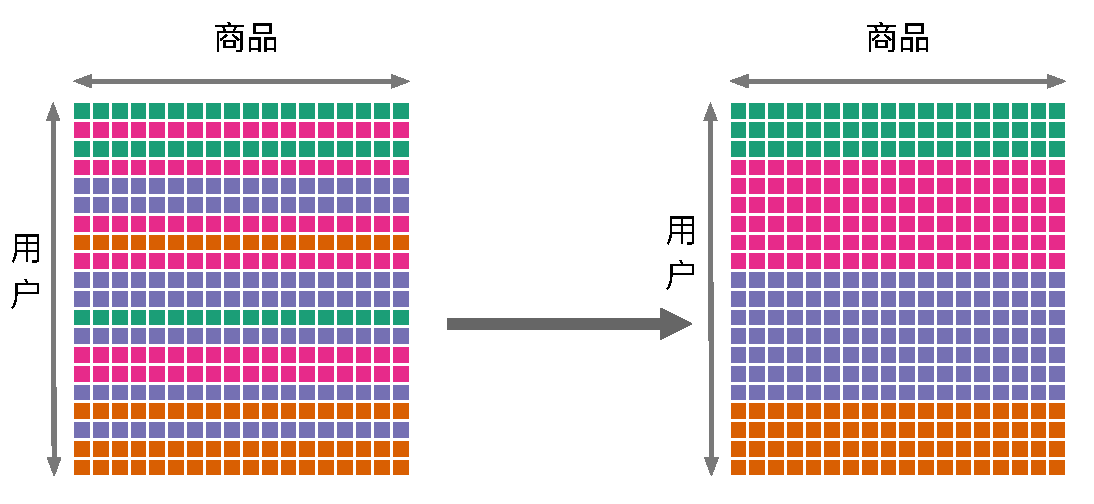
\includegraphics[width=0.75\textwidth]{Fig/lwmf/user}
	\caption{基于用户的局部矩阵分解模型}
	\label{fig-lwmf-user}
\end{figure}

\subsection{基于用户的局部加权矩阵分解}
上述的LWMF方法使用被选中的子矩阵去对\textit{局部}性质进行建模,而忽视了全局信息。特别对于商品推荐问题,应该考虑从所有商品中推荐用户感兴趣的商品。因此,本章节提出一种变种的LWMF方法-基于用户的局部加权矩阵分解,它仅仅从用户角度选择锚点,将所有商品放入子矩阵中。 给定用户集合$\mathcal{P}=\{u_1,u_2,...,u_N\}$ ,以及每个用户$u_i$能覆盖本身和其他一些用户,表示为$\bar{\mathcal{P}^i}=\{u_i, u_{i1}, u_{i2},..., u_{iD}\}$,需要找出一个用户锚点集合$\mathcal{\hat{P}}=\{\hat{u}_1,\hat{u}_2,...,\hat{u}_H\}$去最大化覆盖用户集合,目标函数如下:

\begin{align}
&\max J(\mathcal{\hat{P}}) \sum_{h=1}^{H}\sum_{u_l \in \bar{\mathcal{P}}^h}\alpha^{o_{lh}-1}(1-max_{h'\in\{1,...,h-1\}} E_b(\hat{u}_h,\hat{u}_{h'})) \nonumber \\
&\qquad\qquad\qquad\qquad\qquad\qquad\qquad\qquad\qquad\qquad s.t. |\mathcal{\hat{P}}| = H
\end{align}

显然地,这个基于用户的DCGASC目标函数也是符合次模性质和非减函数。图~\ref{fig-lwmf-user}展示了基于用户的LWMF模型去选择子矩阵的过程。因为不需要考虑商品,基于用户的LWMF会更快地选择用户锚点集合。而且,对于商品推荐来说,基于用户的LWMF模型也相对是比较合适的。作为对基于用户的LWMF模型的比较,本章节也加入了基于商品的LWMF模型,它仅仅考虑商品去选择锚点且把所有用户放入子矩阵中。



%\begin{figure}
%	\centering
%	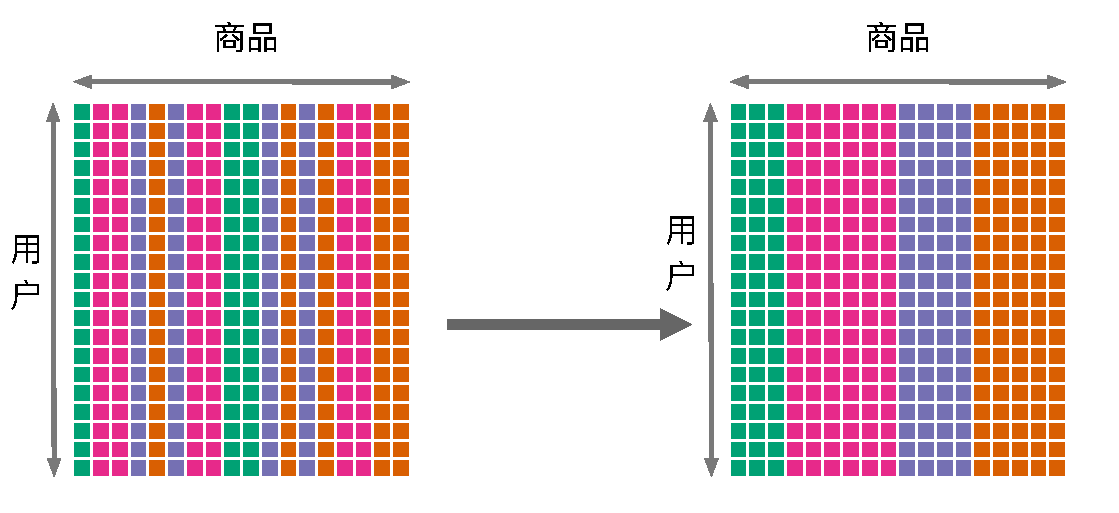
\includegraphics[width=0.7\textwidth]{Fig/lwmf/item}
%	\caption{基于商品的局部矩阵分解}
%	\label{fig-lwmf-item}
%\end{figure}

\section{实验及分析}
\label{sec-lwmf-exp}

本节将在真实世界的隐式反馈数据上评估本章节提出的模型。本小节首先介绍所使用的真实世界数据集和实验设置。随后实验在特定参数下和其他一些著名\textit{商品推荐}模型进行比较,特别是全局的WMF模型。最后实验中也进行了不同锚点数量(也就是不同数量的子矩阵)和不同锚点选择方法下推荐结果的比较。

\subsection{实验设置}
\subsubsection{数据集}
本章工作在实验中选择论文\cite{yuan2013time}中的两个真实世界数据集。一个是新加坡2010年8月到2011年7月的Foursquare签到数据,另外一个是加利福利亚州和内华达州2009年2月到2010年10的签到数据。这两个数据都是非常流行的在线移动位置服务数据,只有签到数据,但没有用户的喜好数据,是非常典型的用户隐式反馈数据。

Foursquare签到数据包含由2,312个用户,5,596个POIs组成的194,108个签到数据,稠密度是$1.50\times10^{-2}$。Gowalla签到数据包含由10,162个用户,24,238个POIs组成的456,967个签到数据,稠密度是$1.86\times10^{-3}$。两个数据集都比较稀疏。表\ref{tab-lwmf-stat}展示了两个数据集更详细的信息。另外,根据用户-地点-签到次数随机将80\%的数据集分割为训练集,剩下的20\%为测试集。对所有方法,本实验分别独立进行5次,最终5次实验的平均值作为最终推荐方法的结果。

\begin{table}
	\centering
	\caption{隐式反馈数据集Gowalla和Foursquare的详细信息}
	\begin{tabular}{|r||r|r|}
		\hline
		& Foursquare & Gowalla \bigstrut\\
		\hline
		\hline
		\#users & 2,321 & 10,162 \bigstrut\\
		\hline
		\#locations & 5,596 & 24,238 \bigstrut\\
		\hline
		\#check-ins & 194,108 & 456,967 \bigstrut\\
		\hline
		avg. \#users per loc. & 34.69 & 18.85 \bigstrut\\
		\hline
		avg. \#loc. per user & 83.63 & 44.97 \bigstrut\\
		\hline
		max \#users per loc. & 695   & 2,195 \bigstrut\\
		\hline
		max \#loc. per user & 311   & 1,113 \bigstrut\\
		\hline
	\end{tabular}%
	\label{tab-lwmf-stat}%
\end{table}%

\subsubsection{参数设置}

接下来,说明本实验中的参数设置。正则化参数$\lambda$设置为10,因为实验中发现该推荐效果对该正则化参数的设置不是非常敏感,10是一个相对较好的数值。置信权重矩阵$\mathbf{W}$中控制权重增量速率的参数$\varepsilon$在数据集Foursquare设置为2,另一个数据集Gowalla上设置为3。用来计算用户之间和商品之间的Epanechanikov核函数的带宽参数设置为$b=0.8$。另外本实验设置锚点选择方法DCGASC的折扣参数$\alpha$为0.4。折扣参数对推荐效果的影响后面有相应的实验结果进行说明。对两个数据集,本实验都选择100个锚点进行最后的矩阵分解。在实验中,可观察到随着锚点数量增多,也就是子矩阵数量增多,推荐效果越好,但是训练时间增加,并且推荐效果增强,收益却减少。实验经验表明100个锚点已经能够得到较好的推荐效果。

\subsubsection{评价标准}
对于评价指标,本实验使用精准率Precision@n和召回率Recall@n衡量模型的推荐性能。对第$u$个用户,本章假设符号$\mathcal{I}^P_u$为他的商品推荐列表,符号$\mathcal{I}^T_u$为该用户在测试数据集中的真实商品列表。Precision@n和召回率Recall@n分别表示为:

\begin{align}
Precision@n &= \frac{1}{N}\sum_{u=1}^{N}\frac{|\mathcal{I}^P_u\bigcap \mathcal{I}^T_u|}{n}\\
Recall@n &= \frac{1}{N}\sum_{u=1}^{N}\frac{|\mathcal{I}^P_u\bigcap \mathcal{I}^T_u|}{|\mathcal{I}^T_u|}
\end{align}
其中$|\mathcal{I}^P_u|$表示列表$\mathcal{I}^P_u$的大小,等于$n$。在基础实验中,选择$n=10$来评价实验结果。

\subsubsection{对比方法}
本实验总共比较7个隐式反馈数据推荐的模型:
\begin{itemize}
	\item MP:这是最基本方法,对目标用户推荐最流行的商品。 
	\item KNN$_u$: 这个是基于用户的协同过滤方法,利用训练集计算用户跟用户之间的相似度,求出$K$\footnote{这里的$K$指的是近邻数量,不是指局部隐藏特征向量的维度。}个最相似的用户对商品的评分之和作为最终预测值。
	\item KNN$_m$: 这个方法跟KNN$_u$类似,是基于商品的协同过滤方法,利用训练集中计算商品跟商品之间的相似度,根据目标用户对其他商品的评测值和跟目标商品之间的相似度计算预测值。特别地,我们设置两个$K$近邻方法的近邻数量为100。
	\item WMF: 该方法为现在最流行的隐式反馈数据top-n商品推荐方法\cite{hu2008collaborative,he2016fast},本文的方法也是基于该方法上提出的,它对缺失数据设置统一的权重,在整个数据集上进行隐藏特征向量参数学习优化。其他基本参数设置和上面参数设置说明一致。
	\item LWMF$_{both}$: 这个方法是本文提出的,利用核函数选择锚点,进而得到子矩阵,来对数据集的局部性质进行建模。
	\item LWMF$_u$: LWMF$_{both}$的一个变种,该方法仅仅考虑用户去选择锚点,并把所有商品放入子矩阵中。
	\item LWMF$_m$:  LWMF$_{both}$的另一个变种,该方法仅仅考虑商品去选择锚点,并把所有用户放入子矩阵中。
\end{itemize}

另外,本实验中也比较了两类不同的锚点选择方法,来研究锚点选择的不同对最终LWMF推荐效果的影响:
\begin{itemize}
	\item 随机选择: 利用均匀分布从训练集中随机选择锚点,和论文\cite{lee2013local,lee2014local}中锚点选择方法类似。
	\item 最大化折扣累积收益锚点集合覆盖锚点选择(DCGASC):利用最大化折扣累积收益锚点集合覆盖函数进行锚点选择。
\end{itemize}

因此LWMF根据锚点选择方法的不同也将分为两个子方法:{LWMF\_random}和{LWMF\_DCGASC}。默认地,不作特别说明,LWMF代表的模型是{LWMF\_DCGASC}方法。

\subsection{实验结果及分析}
本小节将具体介绍在Foursquare和Gowalla两个数据集上的实验结果,主要从以下四个方面进行讨论:
\begin{itemize}
	\item[1.]   各类不同推荐方法的对比;
	\item[2.]  不同锚点数量(即不同子矩阵个数)对本文模型LWMF最终推荐效果的影响;
	\item[3.]  不同锚点选择方法对本文模型LWMF最终推荐效果的影响;
	\item[4.]  折扣参数的不同对本文模型LWMF最终推荐效果的影响。
\end{itemize}

\subsubsection{不同推荐方法的对比} 
% Table generated by Excel2LaTeX from sheet 'Sheet4'
%\begin{table}[htbp]
%	\centering
%	\caption{不同方法准确率和召回率对比,其中行``Improve''代表LWMF对于基线方法WMF推荐效果提高百分比}
%	\subtable[Foursquare数据集]{
%	\begin{tabular}{|c||c|c|c|c|c|c|c|c|}
%		
%		\hline
%		& \multicolumn{2}{c|}{d=5} & \multicolumn{2}{c|}{d=10} & \multicolumn{2}{c|}{d=20} & \multicolumn{2}{c|}{d=40} \bigstrut\\
%		\hline
%		
%		Methods & Precision & Recall & Precision & Recall & Precision & Recall & Precision & Recall \bigstrut\\
%		\hline
%		\hline
%		MP & 0.0615 & 0.0680 & 0.0615 & 0.0680 & 0.0615 & 0.0680 & 0.0615 & 0.0680 \bigstrut\\
%		\hline
%		\hline
%		KNN$_u$  & 0.0741 & 0.8212 & 0.0741 & 0.8212 & 0.0741 & 0.8212 & 0.0741 & 0.8212 \bigstrut\\
%		\hline
%		KNN$_i$  & 0.0698 & 0.7975 & 0.0698 & 0.7975 & 0.0698 & 0.7975 & 0.0698 & 0.7975 \bigstrut\\
%		\hline
%		\hline
%		WMF   & 0.0792 & 0.0905 & 0.0847 & 0.0993 & 0.0844 & 0.0980 & 0.0741 & 0.0922 \bigstrut\\
%		\hline
%		\hline
%		LWMF$_b$ & 0.0823 & 0.0952 & 0.0847 & 0.0995 & 0.0832 & 0.0982 & 0.0828 & 0.0945 \bigstrut\\
%		\hline
%		LWMF$_i$ & \textbf{0.0869} & 0.0962 & 0.0878 & 0.0990 & 0.0893 & 0.1021 & \textbf{0.0907} & 0.1028 \bigstrut\\
%		\hline
%		LWMF$_u$ & 0.0852 & \textbf{0.0999} & \textbf{0.0898} & \textbf{0.1047} & \textbf{0.0915} & \textbf{0.1067} & 0.0902 & \textbf{0.1054} \bigstrut\\
%		\hline
%		\hline
%		Improve & 9.8\% & 10.34\% & 6.03\% & 5.44\% & 8.39\% & 8.85\% & 22.45\% & 14.27\% \bigstrut\\
%		\hline
%	\end{tabular}
%	}\\
%	$\ $\\
%	\hspace{0.5cm}\\
%	\subtable[Gowalla数据集]{
%	\begin{tabular}{|c||c|c|c|c|c|c|c|c|}
%		\hline
%		Gowalla & \multicolumn{2}{c|}{d=5} & \multicolumn{2}{c|}{d=10} & \multicolumn{2}{c|}{d=20} & \multicolumn{2}{c|}{d=40} \bigstrut\\
%		\hline
%		\hline
%		Methods & Precision & Recall & Precision & Recall & Precision & Recall & Precision & Recall \bigstrut\\
%		\hline
%		MP & 0.0203 & 0.0460 & 0.0203 & 0.0460 & 0.0203 & 0.0460 & 0.0203 & 0.0460 \bigstrut\\
%		\hline
%		\hline
%		KNN$_u$  & 0.0552 & 0.1055 & 0.0552 & 0.1055 & 0.0552 & 0.1055 & 0.0552 & 0.1055 \bigstrut\\
%		\hline
%		KNN$_i$  & 0.0587 & 0.1014 & 0.0587 & 0.1014 & 0.0587 & 0.1014 & 0.0587 & 0.1014 \bigstrut\\
%		\hline
%		\hline
%		WMF   & 0.0321 & 0.0664 & 0.0385 & 0.0779 & 0.0442 & 0.0871 & 0.0485 & 0.0953 \bigstrut\\
%		\hline
%		\hline
%		LWMF$_b$ & \textbf{0.0489} & \textbf{0.0923} & \textbf{0.0528} & \textbf{0.0990} & 0.0558 & 0.1035 & 0.0578 & 0.1067 \bigstrut\\
%		\hline
%		LWMF$_i$ & 0.0478 & 0.0884 & 0.0526 & 0.0936 & 0.0565 & 0.1006 & 0.0584 & 0.1034 \bigstrut\\
%		\hline
%		LWMF$_u$ & 0.0445 & 0.0881 & 0.0504 & 0.0989 & \textbf{0.0581} & \textbf{0.1110} & \textbf{0.0623} & \textbf{0.1191} \bigstrut\\
%		\hline
%		\hline
%		Improve & 52.56\% & 39.05\% & 37.10\% & 27.01\% & 31.44\% & 27.41\% & 28.36\% & 25.04\% \bigstrut\\
%		\hline
%	\end{tabular}
%	}%
%	\label{tab-lwmf-foursquare}%
%\end{table}%


\begin{table}
  \centering
  \caption{不同方法的准确率和召回率对比,其中行``Improve''代表LWMF对于基线方法WMF推荐效果提高的百分比}
    \begin{tabular}{|c|c|c|c|c|c|}
    \hline
    \multirow{2}[4]{*}{模型} & \multicolumn{1}{c|}{\multirow{2}[4]{*}{参数}} & \multicolumn{2}{c|}{Foursquare} & \multicolumn{2}{c|}{Gowalla} \bigstrut\\
\cline{3-6}          &       & Precision & Recall & Precision & Recall \bigstrut\\
\hline
  Mostpopular &       & 0.0615 & 0.0680 & 0.0203 & 0.0460 \bigstrut\\
    KNN$_u$  &       & 0.0741 & 0.8212 & 0.0552 & 0.1055 \bigstrut\\
    KNN$_m$  &       & 0.0698 & 0.7975 & 0.0587 & 0.1014 \bigstrut\\
        \hline
    WMF   & \multicolumn{1}{c|}{\multirow{4}[0]{*}{$K=5$}} & 0.0792 & 0.0905 & 0.0321 & 0.0664 \bigstrut\\
    LWMF$_b$ &       & 0.0823 & 0.0952 & 0.0489 & 0.0923 \bigstrut\\
    LWMF$_m$ &       & 0.0869 & 0.0962 & 0.0478 & 0.0884 \bigstrut\\
    LWMF$_u$ &       & 0.0852 & 0.0999 & 0.0445 & 0.0881\bigstrut \\
        \hline
    WMF   & \multicolumn{1}{c|}{\multirow{4}[0]{*}{$K=10$}} & 0.0847 & 0.0993 & 0.0385 & 0.0779 \bigstrut\\
    LWMF$_b$ &       & 0.0847 & 0.0995 & 0.0528 & 0.0990 \bigstrut\\
    LWMF$_m$ &       & 0.0878 & 0.0990 & 0.0526 & 0.0936 \bigstrut\\
    LWMF$_u$ &       & 0.0898 & 0.1047 & 0.0504 & 0.0989 \bigstrut\\
        \hline
    WMF   & \multicolumn{1}{c|}{\multirow{4}[0]{*}{$K=20$}} & 0.0844 & 0.0980 & 0.0442 & 0.0871 \bigstrut\\
    LWMF$_b$ &       & 0.0832 & 0.0982 & 0.0558 & 0.1035 \bigstrut\\
    LWMF$_m$ &       & 0.0893 & 0.1021 & 0.0565 & 0.1006 \bigstrut\\
    LWMF$_u$ &       & \textbf{0.0915} & \textbf{0.1067} & 0.0581 & 0.1110 \bigstrut\\
        \hline
    WMF   & \multicolumn{1}{c|}{\multirow{4}[0]{*}{$K=40$}} & 0.0741 & 0.0922 & 0.0485 & 0.0953 \bigstrut\\
    
    LWMF$_b$ &       & 0.0828 & 0.0945 & 0.0578 & 0.1067 \bigstrut\\
    LWMF$_m$ &       & 0.0907 & 0.1028 & 0.0584 & 0.1034 \bigstrut\\
    LWMF$_u$ &       & 0.0902 & 0.1054 & \textbf{0.0623} & \textbf{0.1191} \bigstrut\\
        \hline
     Improve & & 8.39\% & 8.85\% & 28.36\% & 25.04\% \bigstrut\\
    \hline
    \end{tabular}%
  \label{tab-lwmf-foursquare}%
\end{table}%

表\ref{tab-lwmf-foursquare}列出了在数据集Foursquare和Gowalla上上述7个\textit{商品推荐}模型的精准率和召回率。跟之前文献实验结果一样,WMF在维度合适的情况下,性能比K近邻算法要好。尽管在WMF隐藏特征向量维度$K$较低时,KNN$_u$和KNN$_m$效果较好,但是随着维度$K$的增大,WMF的推荐效果逐渐接近并超过KNN$_u$和KNN$_m$。其次,LWMF在隐藏特征向量维度一样的情况下推荐准确率一般要优于WMF。另外,本章节提出的模型LWMF要优于WMF,这跟做\textit{评分预测}的论文\cite{lee2013local}中结果一致。从表中还可以看出,WMF和LWMF的推荐效果随着隐藏特征向量维度$K$的增大而提高。不过在数据集Foursquare上,维度$K$达到40时,两者的性能反而有所下降,这表明当维度在$40$维时,模型已经过拟合了。另外一方面,数据集Gowalla上的实验结果表明维度$K$在40(或者大于40)时效果最好。因此在接下来的实验中,在数据集Foursquare上设置隐藏特征向量维度为$K=20$而在数据集Gowalla上设置为40。很显然地,LWMF$_b$及其两个变种方法LWMF$_u$和LWMF$_m$在精准率和召回率上在所有维度($K=5,10,20, 40$)上都要优于WMF。特别是Gowalla数据集上,LWMF$_u$优于WMF至少25\%以上。在维度$K$设置为5时,LWMF$_{b}$的精准率甚至高出WMF 52个百分点。这些显著的提高表明在隐式反馈数据上对局部信息建模能够提高推荐准确率。特别在签到数据集中,每个城市中会有一些商区,而商业POIs在每个商区中有着天然的地理上相近,并且用户也喜欢去距离较近的POIs,方便用户本身访问。对于本章提出的模型LWMF及其两个变种的对比中,可以发现它们之间的推荐效果比较相近。但是在全局角度看,基于用户的LWMF$_u$要略微优于其他两个方法。LWMF$_u$基于用户进行推荐,利用全局商品作为子矩阵商品,对于基于商品的LWMF$_m$看上去更为合理一些。因此在接下来的对比实验中都以基于用户的LWMF$_u$作为LWMF的默认方法。

\subsubsection{不同锚点数量推荐结果对比} 
\begin{figure}
	\centering
	\subfigure[Precsion on Foursquare]{
		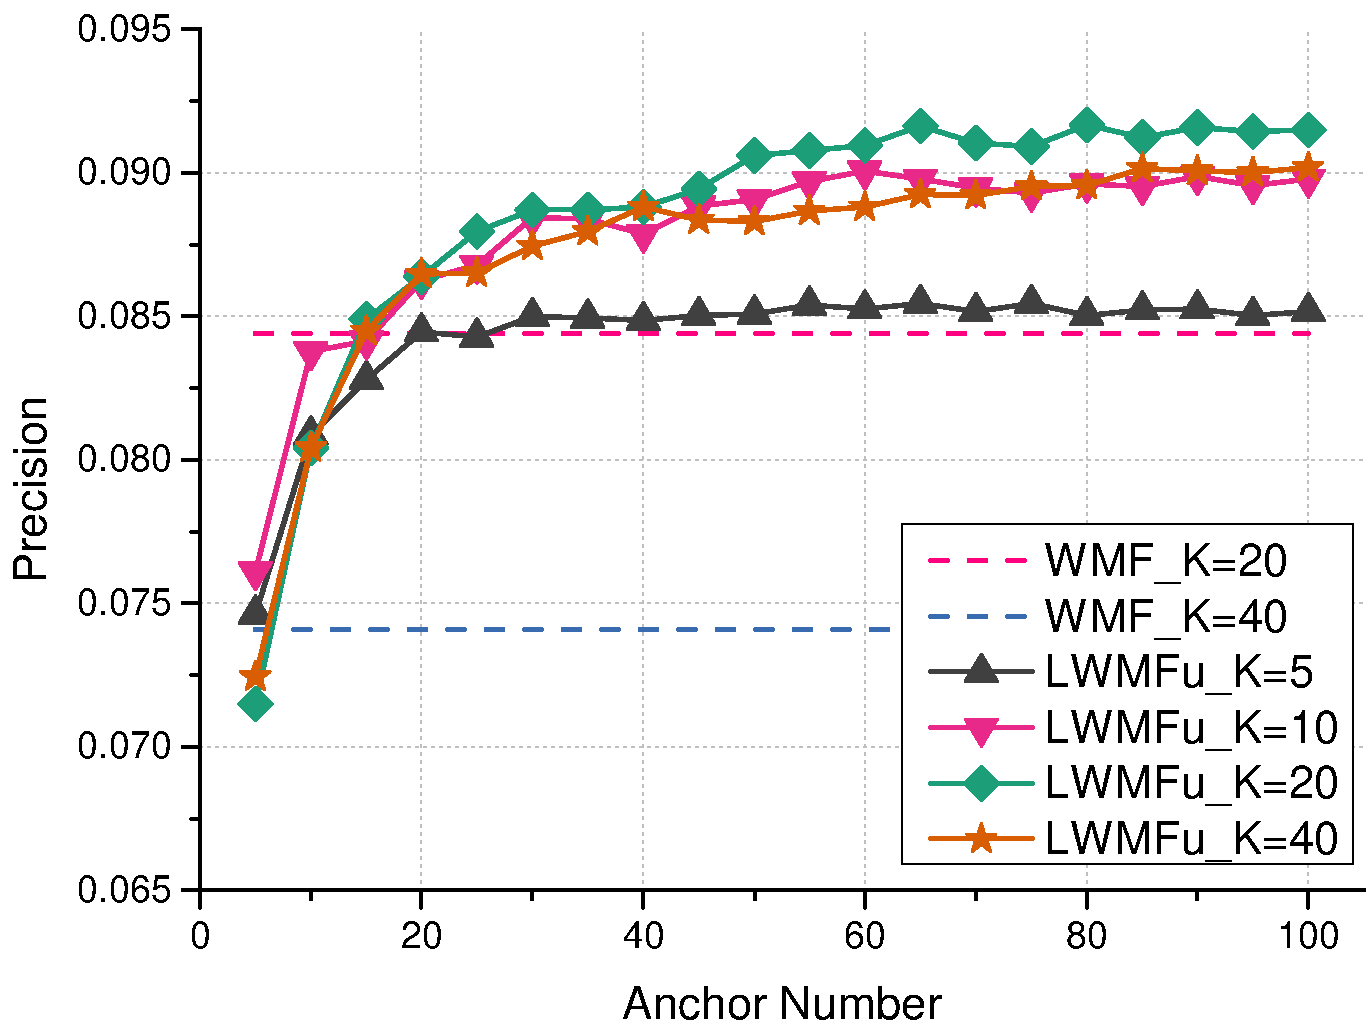
\includegraphics[width=0.486\textwidth]{Fig/lwmf/faprecision}}
	\hspace{0.0cm}
	\subfigure[Recall on Foursquare]{
		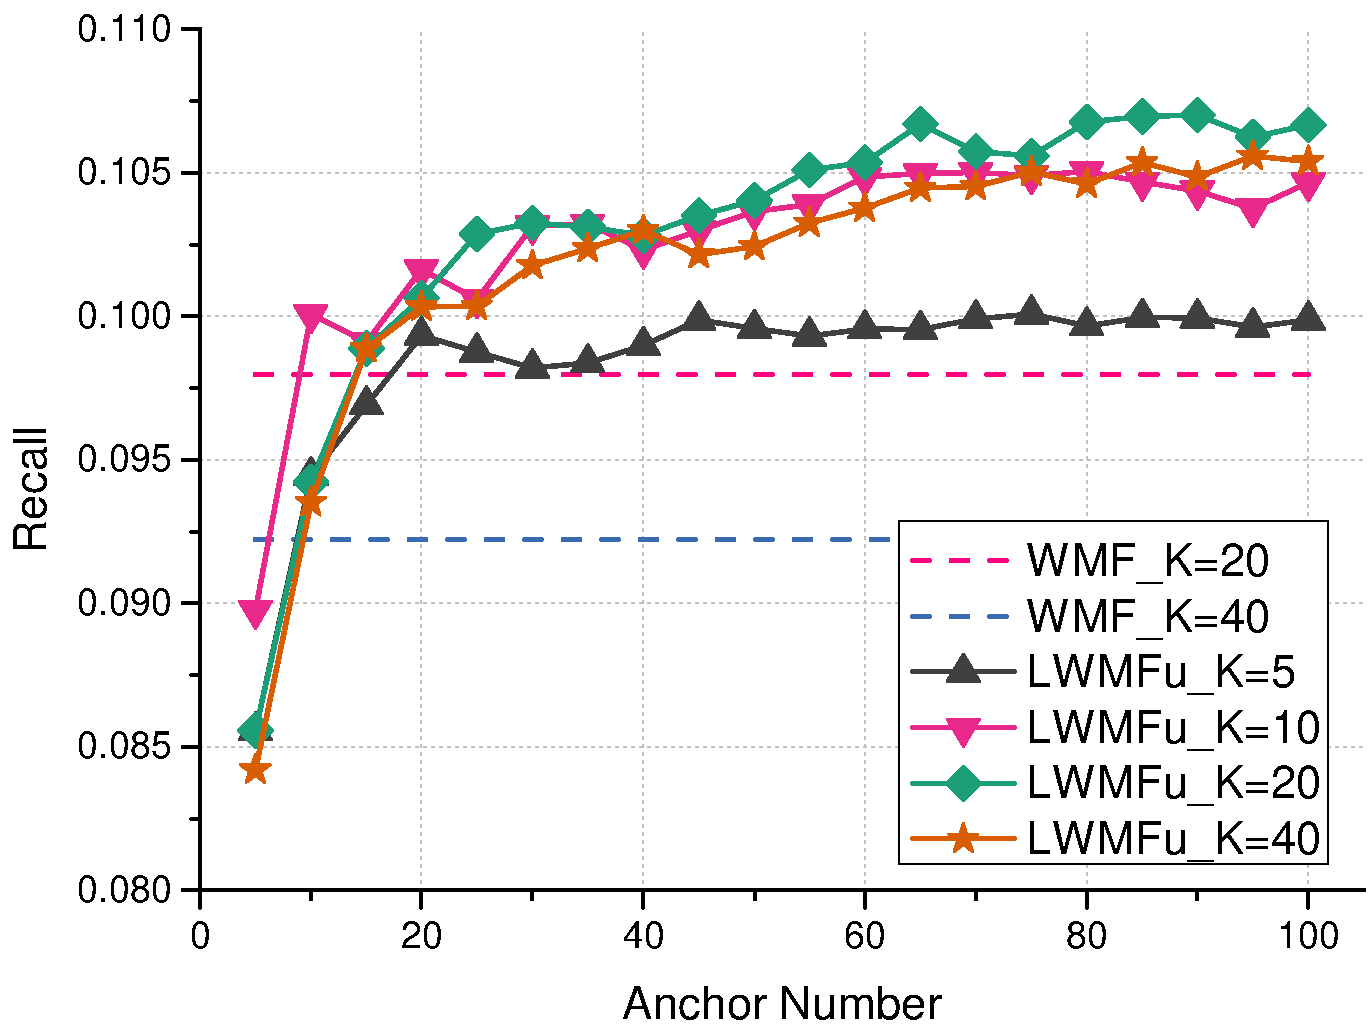
\includegraphics[width=0.486\textwidth]{Fig/lwmf/farecall}}
	\subfigure[Precsion on Gowalla]{
		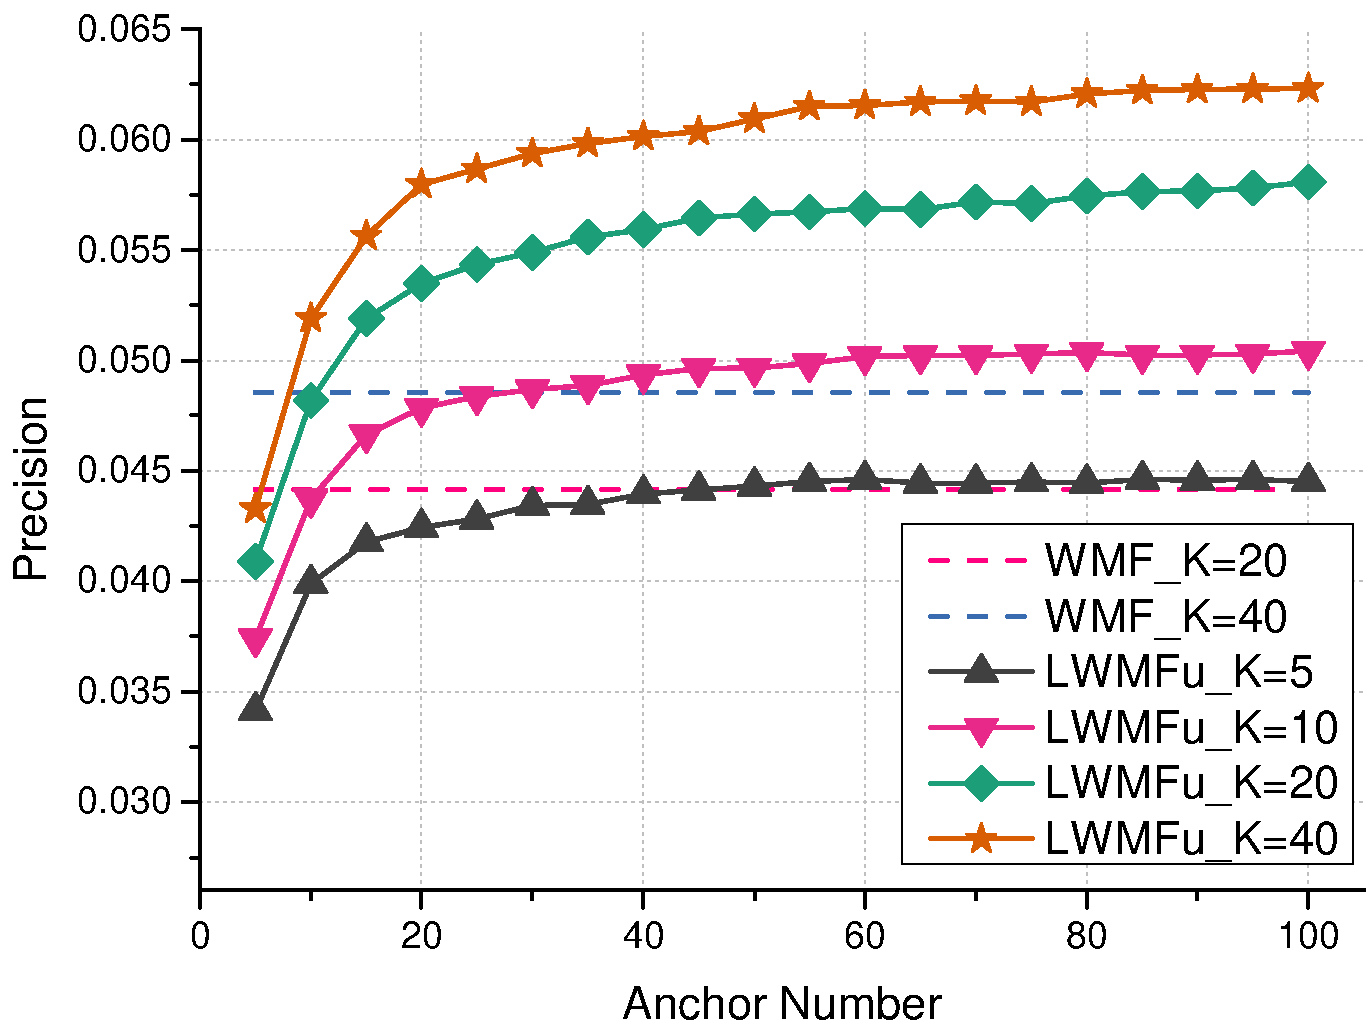
\includegraphics[width=0.486\textwidth]{Fig/lwmf/gowalla_precision}}
	\hspace{0.0cm}
	\subfigure[Recall on Gowalla]{
		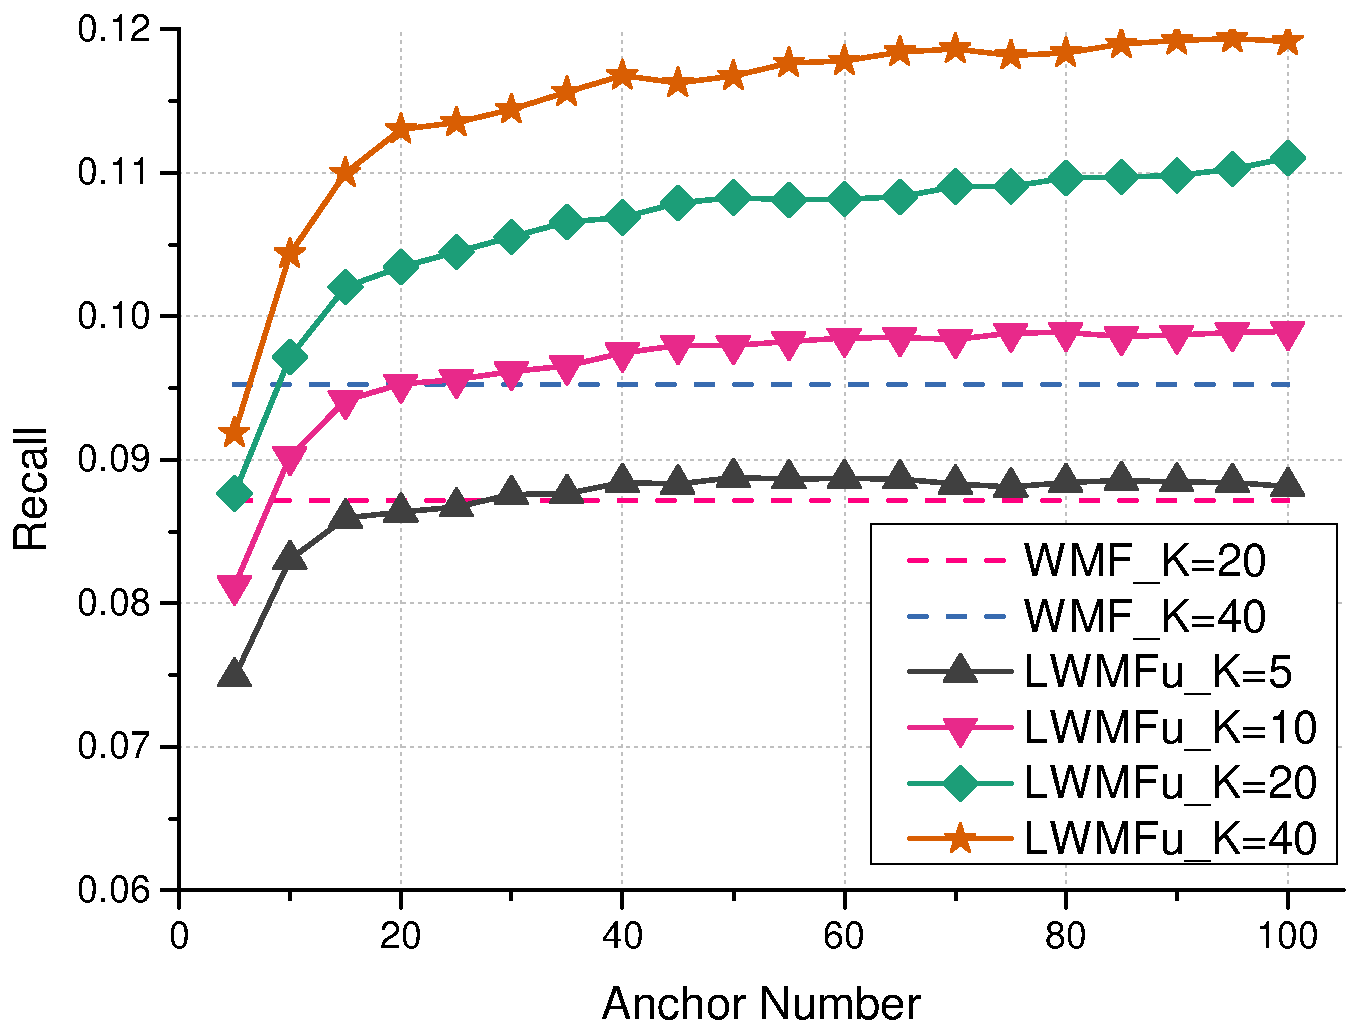
\includegraphics[width=0.486\textwidth]{Fig/lwmf/garecall}}
	
	\caption{不同锚点数量的推荐结果对比}
	\label{fig-lwmf-anchor}
\end{figure}

图~\ref{fig-lwmf-anchor}展示了不同锚点数量(即不同子矩阵个数)对本章节模型LWMF最终推荐效果的影响。在两个数据集上,LWMF的精准率和召回率都随着隐藏特征向量维度$K$提高而提高,并且LWMF在维度$K$大于等于10以后,推荐效果就优于WMF。当锚点数量$H$大于20,也就是说子矩阵数量大于20时,LWMF的推荐效果开始超过WMF,并且随着锚点数量的增多,效果越好,但同时效果边际收益却在下降。并且因为锚点的增加,子矩阵变多,训练模型的时间也会随着增加,因此用户可以根据本身时间和推荐精度需求,动态选择锚点数量。途中还可以看出当锚点数量$H$等于50的时候可以得到相对较好的实验结果。使用基于元素级最小二乘算法的WMF每一轮迭代的复杂度为$O(NK^2+MK^2+|\mathbf{R}|K)$,而整个LWMF模型每一轮迭代的复杂度为$O(\hat{H}(NK^2+MK^2+|\mathbf{R}|K))$,两者的复杂度相差$\hat{H}$倍。两个数据集中,每个子矩阵大小平均是原始矩阵的10\%左右。因此每个子矩阵的训练时间是远快于整个矩阵的分解训练。当子矩阵个数为50时,训练时间大概是WMF的5倍左右,基于推荐效果的提高,LWMF的训练时间还是能够接受的,并且LWMF经过子矩阵选择后,有着比WMF更好的数据和模型并行度,易于并行扩展。

\subsubsection{不同锚点选择方法推荐结果对比}
\begin{figure}
	\centering
	\subfigure[Precsion on Foursquare]{
		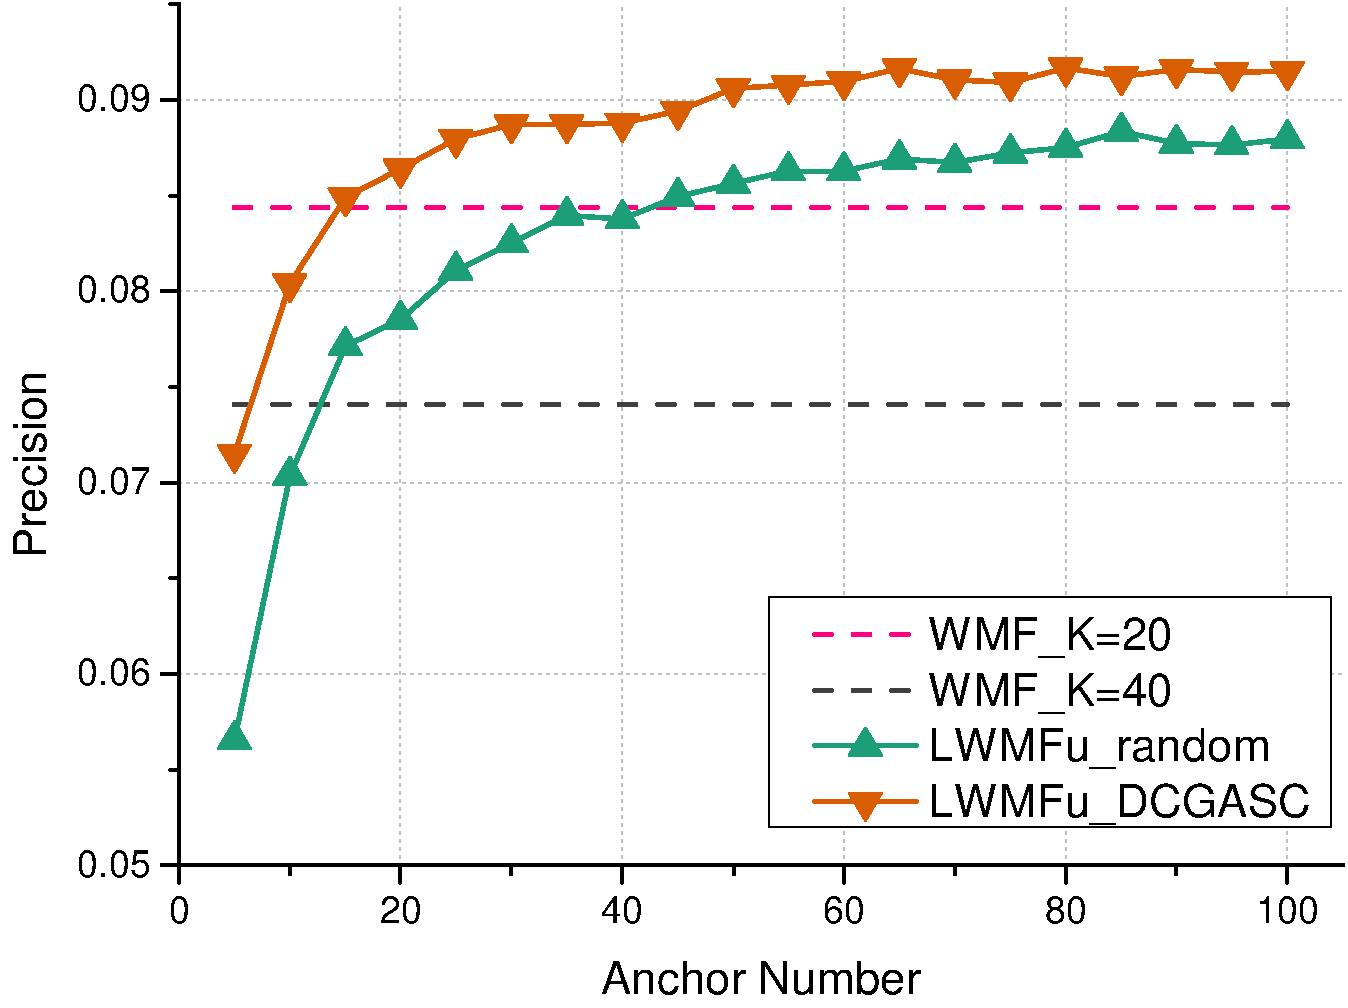
\includegraphics[width=0.486\textwidth]{Fig/lwmf/fradomprecision}}
	\hspace{0.0cm}
	\subfigure[Recall on Foursquare]{
		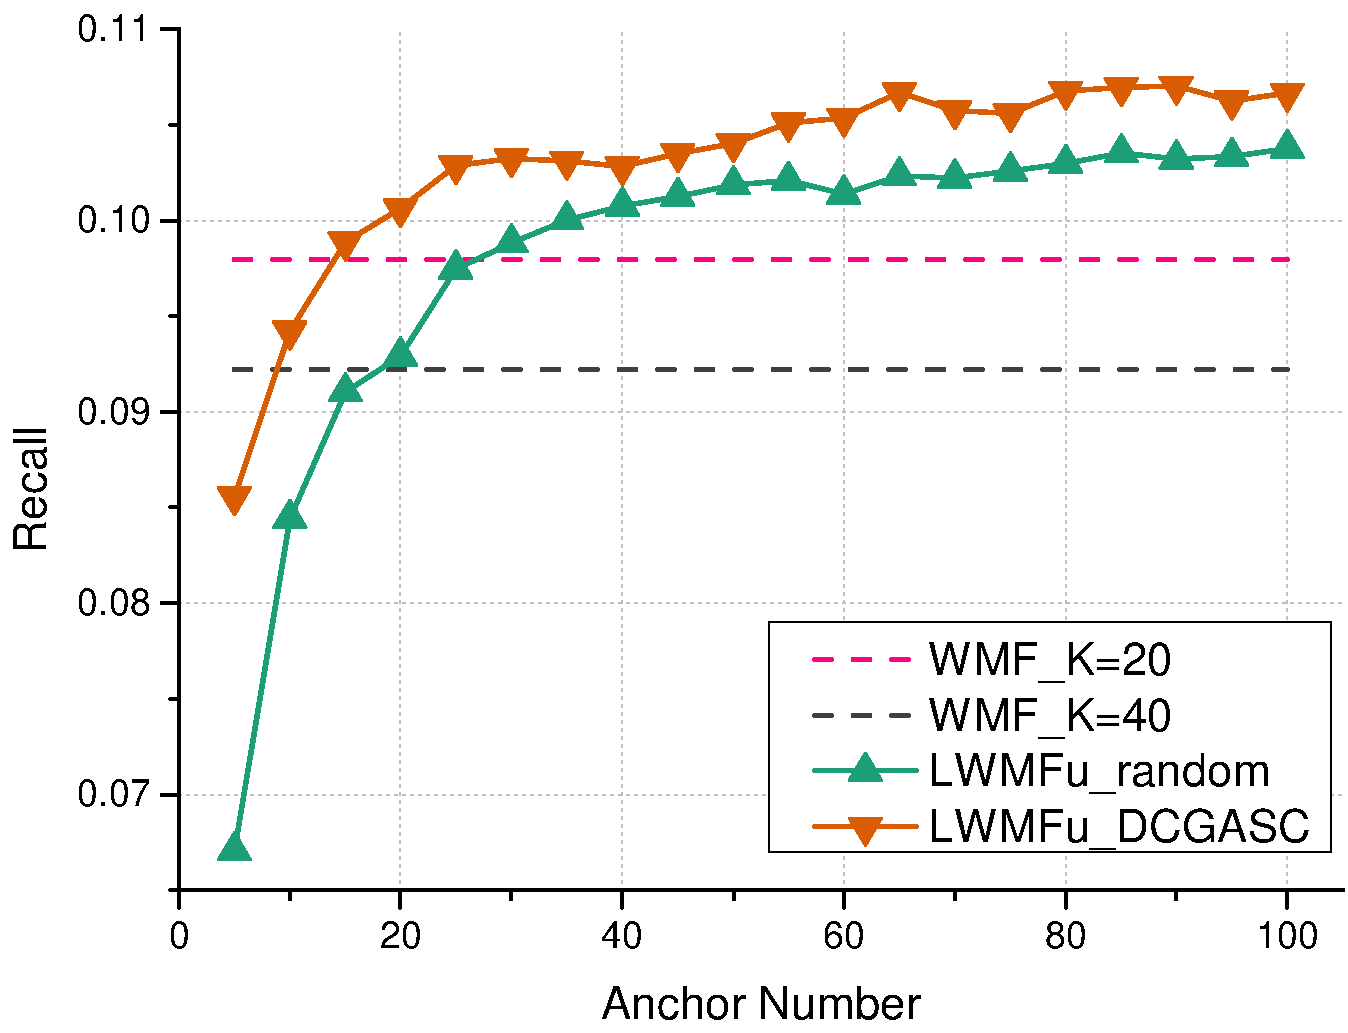
\includegraphics[width=0.486\textwidth]{Fig/lwmf/frandomrecall}}
	\subfigure[Precsion on Gowalla]{
		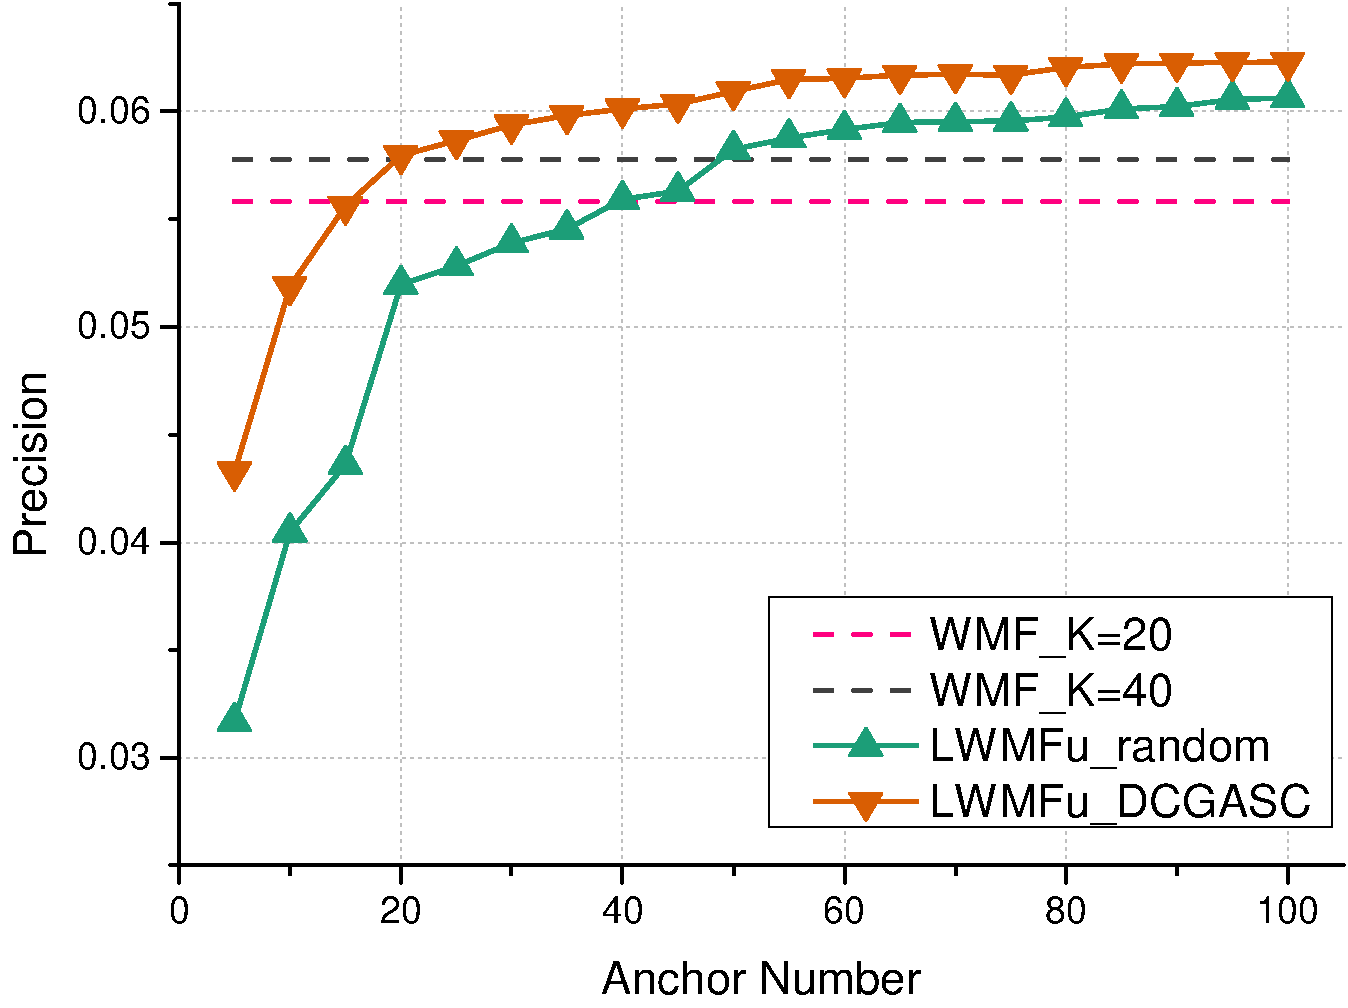
\includegraphics[width=0.486\textwidth]{Fig/lwmf/grandomprecision}}
	\hspace{0.0cm}
	\subfigure[Recall on Gowalla]{
		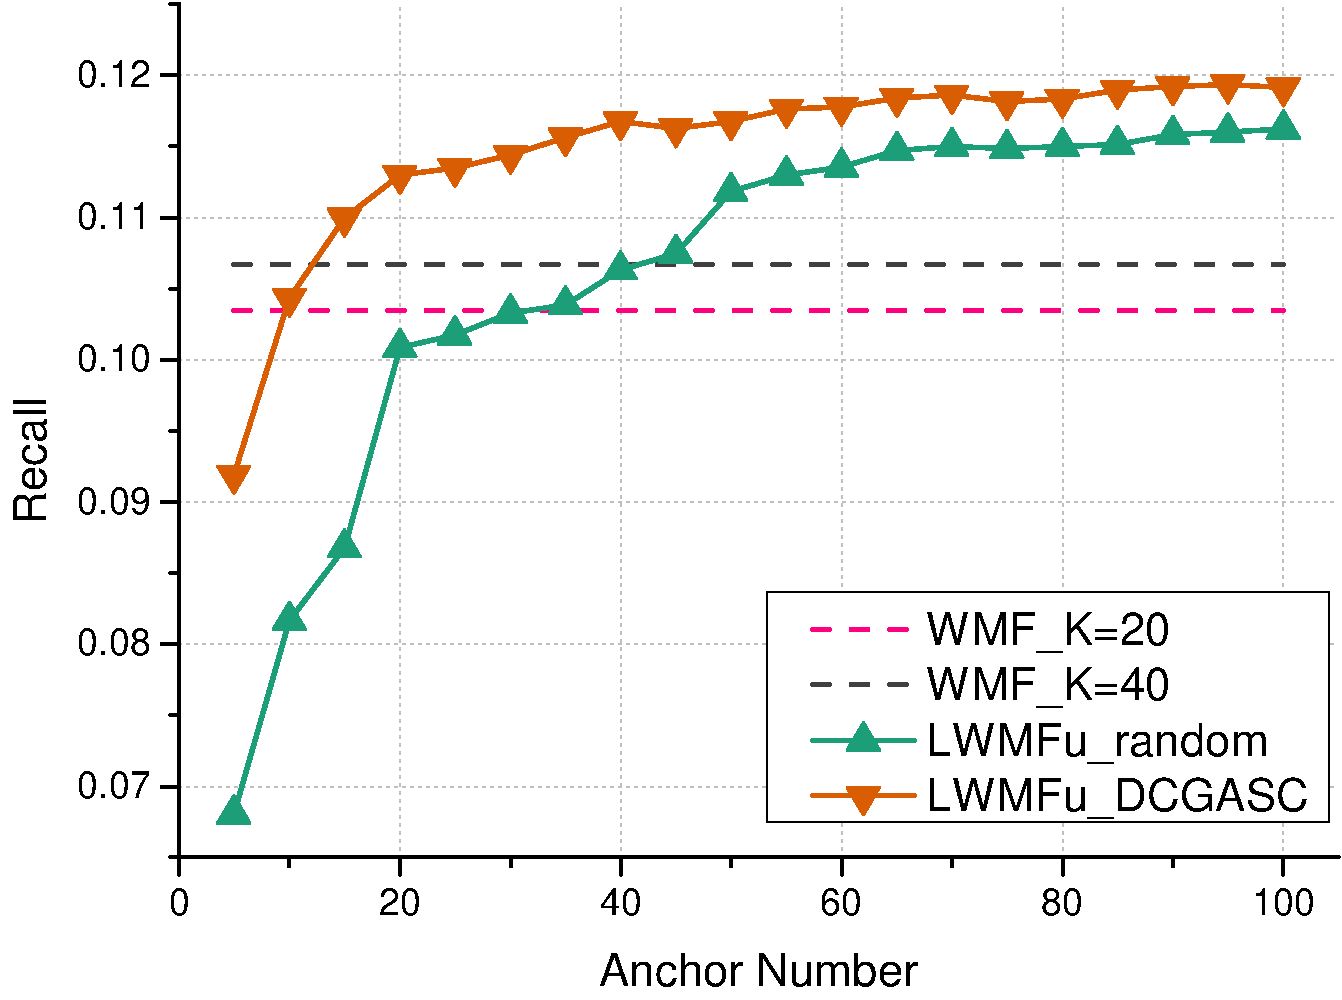
\includegraphics[width=0.486\textwidth]{Fig/lwmf/grandomrecall}}
	
	\caption{不同锚点选择方法的推荐结果对比}
	\label{fig-lwmf-random}
\end{figure}

本小节实验展示了不同锚点选择方法对本文模型LWMF最终推荐效果的影响。本实验中,DCGASC折扣系数$\alpha$设置为0.4,隐藏特征向量维度$K$在数据集Foursquare设置为20,数据集Gowalla上的维度设置为40。从图~\ref{fig-lwmf-random}中可以看出,锚点数量从0到100,基于用户选择锚点的{LWMF$_u$}的精准率和召回率都要优于基于训练集随机选择锚点的LWMF。不过随着锚点数量的增加,两者间的差距越来越小。可以肯定地是,随着锚点数量越来越多,两者性能将会差不多。极端情况下选取所有候选数据点作为锚点来选择子矩阵,{LWMF$_u$}
和{LWMF$_u$\_Random}是一样的。但考虑到锚点数量影响模型的训练时间,锚点数量越多(子矩阵越多),训练时间越久,因此从训练时间角度来看锚点数量越少越好。总体来看,{LWMF$_u$}在两个数据集上都要优于{LWMF$_u$\_Random}。

\subsubsection{不同折扣参数推荐结果对比}
\begin{figure}
	\centering
	\subfigure[Precsion on Foursquare]{
		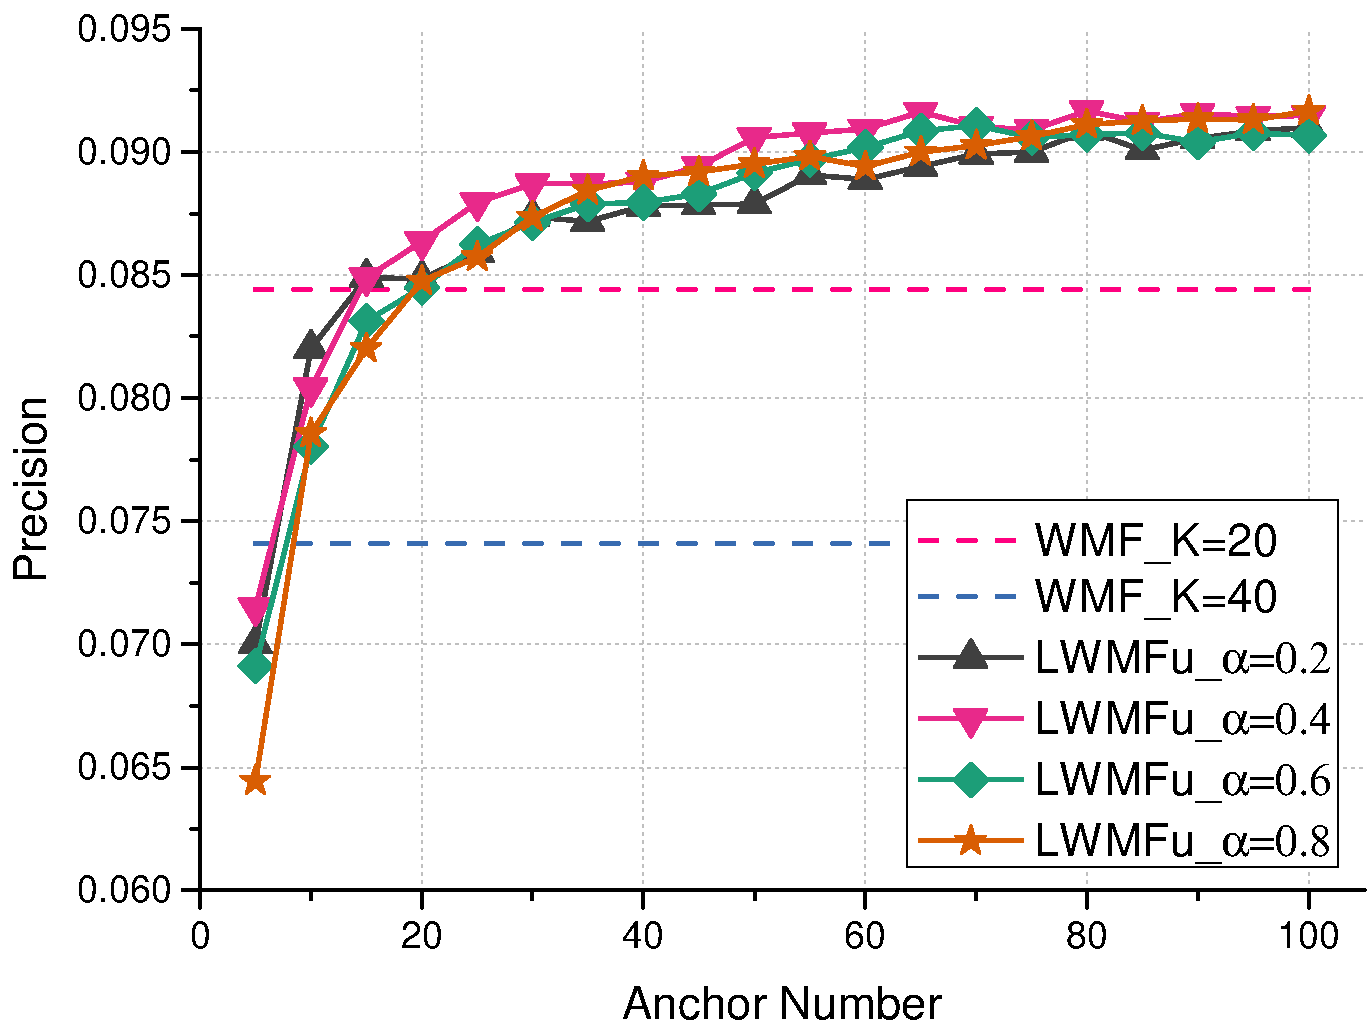
\includegraphics[width=0.486\textwidth]{Fig/lwmf/falphaprecision}}
	\hspace{0.0cm}
	\subfigure[Recall on Foursquare]{
		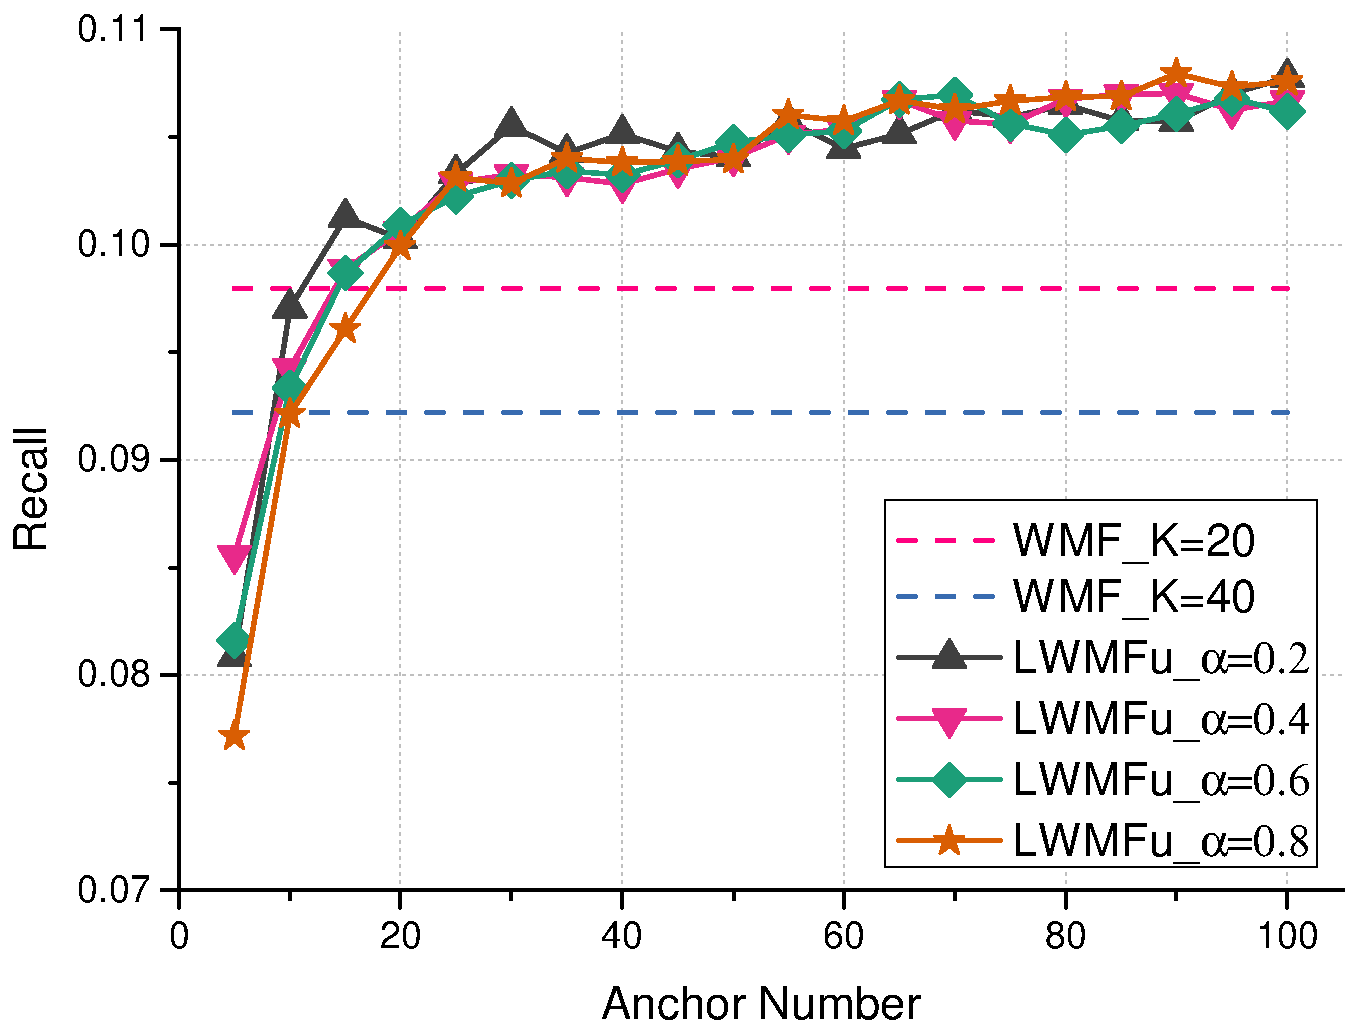
\includegraphics[width=0.486\textwidth]{Fig/lwmf/falpharecall}}
	\subfigure[Precsion on Gowalla]{
		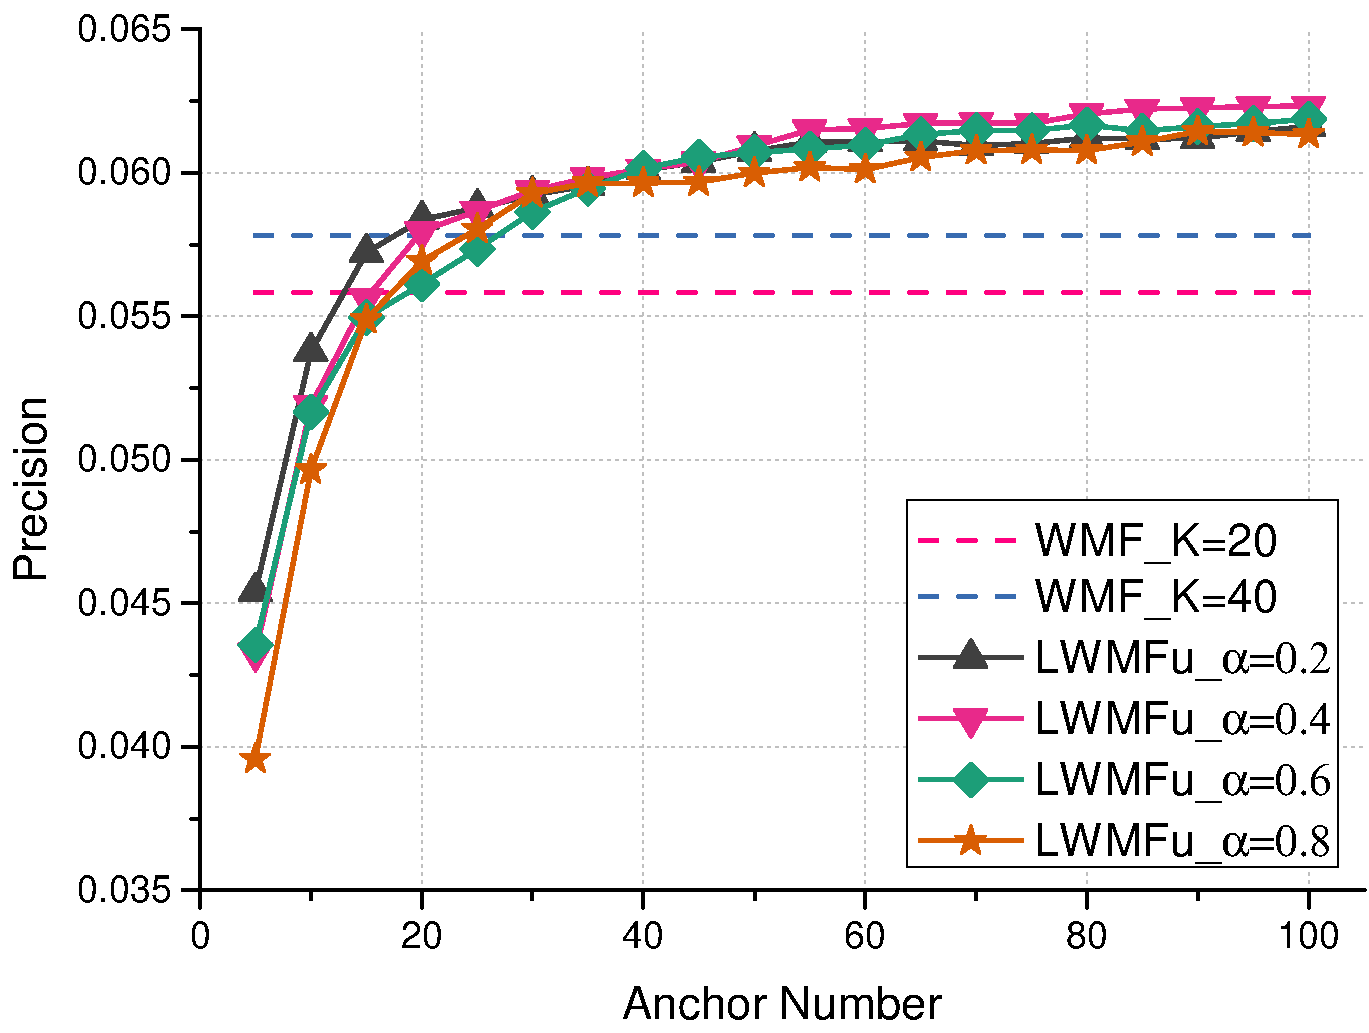
\includegraphics[width=0.486\textwidth]{Fig/lwmf/galphaprecision}}
	\hspace{0.0cm}
	\subfigure[Recall on Gowalla]{
		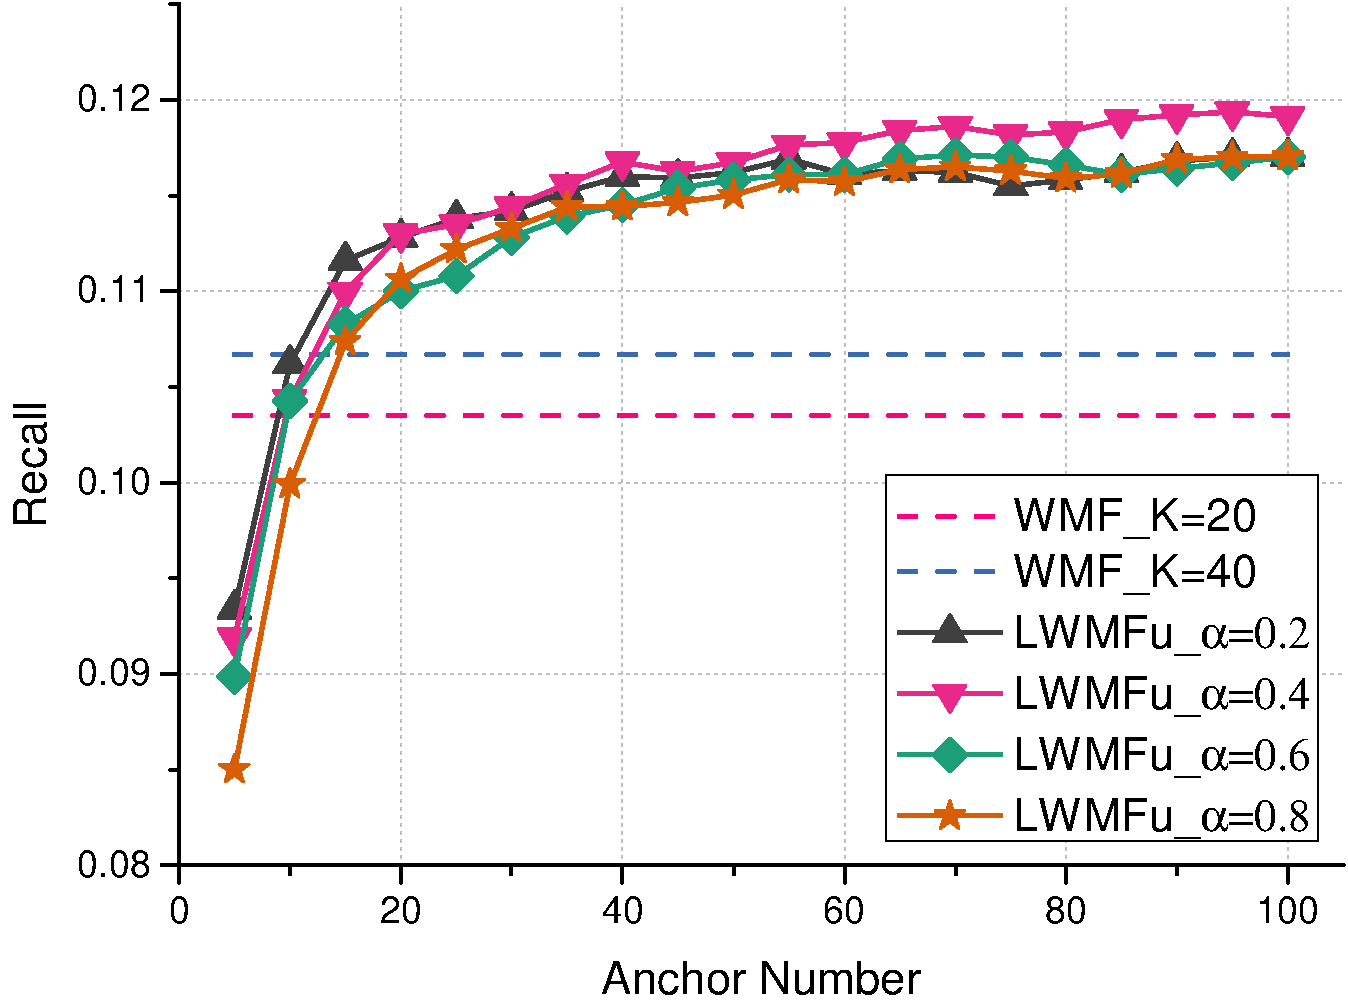
\includegraphics[width=0.486\textwidth]{Fig/lwmf/galpharecall}}
	
	\caption{不同折扣参数的推荐结果对比}
	\label{fig-lwmf-alpha}
\end{figure}

本小节研究折扣参数的不同对本文模型{LWMF$_u$}最终推荐效果的影响。跟上小节一样,隐藏特征向量维度$K$在数据集Foursquare设置为20,数据集Gowalla上设置为40。对于折扣系数$\alpha$,我们验证了范围$[0.1,0.9]$之间以0.1为间隔的推荐结果。因为不同的折扣参数,推荐的精准率和召回率较为相似,我们在本文中只画出$\alpha \in \{0.2,0.4,0.6,0.8\}$的结果曲线,如图~\ref{fig-lwmf-alpha}所示。可以看出,四个不同折扣参数之间的推荐效果差距是非常小的。相对来说,折扣参数$\alpha = 0.4$是略微优于其他参数设置。总得来说,LWMF的推荐性能对折扣参数的设置不敏感,主要依靠于锚点数量、锚点的选择方法以及隐藏特征向量维度三个方面。

\section{本章小结}
本章针对隐式反馈数据上的\textit{商品推荐}任务提出局部加权矩阵分解模型(LWMF),将整个训练数据矩阵分成一系列内部数据相似的子矩阵,然后对每个子矩阵利用加权矩阵分解得到用户和商品隐藏特征向量,最后利用隐藏向量对每个预测子矩阵进行加权平均近似原始矩阵。此外,本章工作设计了高效的子矩阵选择算法建模数据的局部信息,并改进了交替最小二乘算法进行子矩阵加权分解,刻画用户和商品的局部内在特征。同时,LWMF带来两个额外好处,缓解了数据稀疏性问题和更好地进行分布式矩阵分解。 最后,在两个真实数据集的实验表明相对于传统的WMF模型,LWMF能够有效地提高在隐式反馈数据数据上的商品推荐效果。

\clearpage
\phantom{s}
\clearpage